\documentclass[en,license=none]{../../../eplsummary}

\usepackage{multirow}
\usepackage{multicol}
\usepackage{graphicx}
\usepackage{../../../eplunits}
\usepackage{../../../eplcode}
% Footnote in tabular
\usepackage{footnote}
\makesavenoteenv{tabular}
\makesavenoteenv{table}

\newcommand\sifs{\textnormal{SIFS}}
\newcommand\difs{\textnormal{DIFS}}
\newcommand\eifs{\textnormal{EIFS}}
\lstset{language={C}}

\hypertitle{Computer Networks: Information transfer}{5}{INGI}{1341}
{Nicolas Houtain\and Benoît Legat\and Gorby Nicolas Ndonda Kabasele\and Gilles
Peiffer\and Florian Thuin}
{Olivier Bonaventure}

\graphicspath{{images/}}
\lstset{inputpath=algorithm}

\section{Terminology}

\begin{description}
    \item[ADSL]: \textit{Asymmetric Digital Subscriber Line}. The working principle here is to have high download speeds but low upload speeds on the consumer's end.
    \item[ARP]: \textit{Address Resolution Protocol}.
    \item[BPDU]: \textit{Bridge Protocol Data Unit}.
    \item[CRC]: \textit{Cyclical Redundancy Check}.
    \item[\difs{}]: \textit{DCF Interframe Space}. If a station detects the medium has been continuously idle for a duration of \difs{},
    and the last frame transmission was successful (no corruption or error),
    it is then allowed to transmit a frame.
    If the last transmission contained an error,
    the station must wait for a duration of \eifs{} for any frame (re)transmission.
    \difs{} respects the following relation :
    $\difs{} = \sifs{} + (2 \cdot \textnormal{Slot time}$).
    \item[DNS]: \textit{Domain Name System}. Naming system for associating various information (such as an IP address) with a domain name.
    \item[\eifs{}]: \textit{Extended Interframe Space}. Similar to \difs{} but is only activated if the last frame contains an error.
    The \eifs{} duration is defined as follows:
    \[\eifs{} = \textnormal{Transmission time of Ack frame at lowest physical rate (or bit rate)} + \sifs{} + \difs{}.\]
    \item[HTTP]: \textit{HyperText Transfer Protocol}.
    \item[IEEE]: \textit{Institute of Electrical and Electronics Engineers}.
    \item[LAN]: \textit{Local Area Network}.
    \item[MSL]: \textit{Maximum Segment Life}.
    \item[MTU]: \textit{Maximum Transmission Unit} Maximum size of a protocol data unit that can be communicated in a single network layer transaction.
    \item[Path MTU]: Maximum transmission unit size on the network between two Internet Protocol hosts.
    \item[PDU]: \textit{Protocol data unit}. Information that is transmitted as a single unit among peer entities of a computer network.
    \item[RIFS]: \textit{Reduced Interframe Space}.
    \item[SDU]: \textit{Service Data Unit}.
    \item[\sifs{}]: \textit{Short Interframe Space}. Amount of time in microseconds required for a wireless interface to process a received frame and to respond with a response frame.
    More precisely, it is the time interval between the last bit of the transmitted frame and the first bit of the corresponding response frame.
    \item[TLV]: \textit{Type-length-value}. Encoding scheme used for optional information elements in a certain protocol.
    The first byte is a type,
    the second byte is the size of the value field
    and the rest is the value field.
\end{description}

\section{Layers}

The different layers are represented by \tabref{layers}.
A router only has 3 layers: Network, Datalink and Physical.
The TCP/IP model combines the Datalink and Physical layer into a Link layer.
\begin{table}[!ht]
  \centering
  \begin{tabular}{|c|c|c|p{4cm}|c|c|}
    \hline
    \multicolumn{3}{|c|}{Layers} & Protocols & PDU\footnote{Protocol Data Unit}
    & Id\footnote{I know it is a bit of an overgeneralization\dots}\\
    \cline{1-3}
    CNP3 & TCP/IP & OSI & & & \\
    \hline
    \multirow{3}{*}{Application} & \multirow{3}{*}{Application}             &
    Application  & BGP, DHCP, DNS, FTP, HTTP, NFS, NTP, RIP, SMTP, SNMP, Telnet
    & ADU & \\
    \cline{3-6}
                                 &                                          &
                                 Presentation & MIME, XDR, SSL & & \\
    \cline{3-6}
                                 &                                          &
                                 Session      & RTP, TLS & SDU & \\
    \hline
    Transport                    & Transport                                &
    Transport    & UDP, MPTCP, TCP, SCTP & segment & Port\\
    \hline
    Network                      & Internet                                 &
    Network      & ICMP, IPsec, IPv4, IPv6, IPX, MPLS\footnote{MultiProtocol Label Switching operates at a layer that is generally considered to lie between traditional definitions of layer 2 (data link layer) and layer 3 (network layer),
    and thus is often referred to as a ``layer 2.5'' protocol.}
    & packet & IP\\
    \hline
    Datalink                     & \multirow{2}{*}{Link}                    &
    Datalink     & IEEE 802.3 (Ethernet), IEEE 802.4, IEEE 802.5, ATM, ARP,
    Frame Relay, HDLC, IS-IS, LAPB, LLC, MAC, OSPF, PPP, SLIP & frame & MAC\\
    \cline{1-1}
    \cline{3-6}
    Physical                     &                                          &
    Physical     & DSL, IEEE 802.3 (Ethernet), IEEE 802.11 (WiFi), ISDN, Modems
    & bit & \\
    \hline
  \end{tabular}
  \caption{This table contains all the protocols of
  \cite{bonaventure2011computer}. See \cite{wiki:osimodel} for more protocols.}
  \label{tab:layers}
\end{table}

\begin{table}[!ht]
\centering
	\begin{tabular}{|c|l|l|}
	\hline
	Layer&Feature&Protocol \\
	\hline
    \multirow{2}{*}{Application}&&BGP, DHCP, DNS,\\
                                &&HTTP, FTP\\
	\hline
	\multirow{2}{*}{Transport}&Connectionless unreliable (CRC)&UDP\\
                              &connection-oriented reliable (graceful)&TCP,
                              STCP\\
	\hline
	\multirow{2}{*}{Network}&Connectionless unreliable(datagram)&IPv6, IPv4,
     OSPF, RIP\\
                            &connection-oriented(virtual circuit)&\\
	\hline
	\multirow{2}{*}{Datalink}&Unreliable (WiFi), uses window-based
     protocol&WiFi\\
                             &Reliable(Wires)&Ethernet, SLIP, PPP\\
	\hline
	Physical&Unreliable (add/delete/change bit)&\\
	\hline
	\end{tabular}
\end{table}

\begin{myexem}
  An HTTPS request will use the following protocols in each layer of the OSI model:
  \begin{description}
    \item[Application] HTTP,
    \item[Presentation] SSL,
    \item[Session] TLS,
    \item[Transport] TCP,
    \item[Network] IPv6,
    \item[Datalink] IEEE 802.3 (Ethernet),
    \item[Physical] IEEE 802.3 or IEEE 802.11 (Wireless Local Area Network).
  \end{description}
\end{myexem}

\subsection{Physical Layer}
The Physical Layer service is provided by
\begin{itemize}
  \item \textbf{Electrical cable} twisted pairs or coaxial cables;
  \item \textbf{Optical fiber} multimode or monomode;
  \item \textbf{Wireless} laser for point-to-point and
  radio-based for spread signal (e.g. WiFi).
\end{itemize}
Its PDU is the bit and the following terms are used
\begin{itemize}
    \item \textbf{Bit rate}: Expressed in bits/sec;
    \item \textbf{Bandwith}: Range of frequency usable.
\end{itemize}

\subsubsection{Characteristic}

It is \textit{not perfect} (unreliable),
and to us it is like a black box with these characteristics:
\begin{itemize}
    \item \textcolor{red}{changes} the value of a bit
    (\textit{because of electromagnetic interference});
    \item delivers \textcolor{red}{more or fewer} bits than requested
    (\textit{because of an imprecise clock frequency}).
\end{itemize}

\paragraph{Manchester encoding}
It's an encoding that consists in dividing time in fixed length periods.
To send a 1, the voltage must be high in the first half of a period and then become low.
For zero, it's the opposite.
It uses the InvH (high voltage during last period) and InvB symbols as special markers.

\subsection{Datalink Layer}
The PDU of the Datalink Layer service is a \textbf{frame}
(\textit{sequence of bits with a particular syntax or structure})
because we want to share data blocks.
A frame can be separated into 3 parts:
\begin{itemize}
    \item \textbf{Header} It contains a flag that tells whether it's an \textcolor{red}{ACK} or \textcolor{red}{DATA},
    a \textcolor{red}{sequence number}
    and sometimes the length of the payload.
  \item \textbf{Payload} It contains the information that needs to be transmitted.
  \item \textbf{Error-detecting code} It allows the receiver to detect transmission errors.
    It is either
    \begin{itemize}
        \item a \textsc{hamming code} which is simply a parity bit,
        it can only detect an odd number of errors;
        \item a \textsc{checksum} such as
        the Internet checksum chosen by the TCP/IP community
        and the Fletcher checksum chosen by the OSI community;
        \item or a \textsc{Cyclic Redundancy Check} (CRC).
        It was slow to implement in software before 1995 and the publication of \cite{feldmeier1995fast}.
        It is now preferred since it has better error detection \cite{stone1998performance}.
        An $n$-bit CRC will detect errors bursts not longer than $n$ bits
        and will detect a fraction ($1-2^{-n}$) of all longer error bursts.
        \item a \textsc{hash function} like MD5 or SHA.
        However, these are built to be collision resistant against an active adversary, not random modifications.
        They are also a lot slower than CRC or checksums
        so they are only used in cryptography.
    \end{itemize}
  \item \textbf{Error-correcting code} It allows the receiver to correct transmission errors.
  No widely used datalink protocol uses this.
\end{itemize}

\subsubsection{Framing}

The separation of frames is done using \emph{bit stuffing} or \emph{character stuffing}.

\begin{description}
    \item[Bit stuffing]: \textbf{01111110} is a frame \textcolor{red}{boundary marker}, so it can't be used inside the transmitted frames.
    \textit{Adds a 0 after 5 consecutive 1's to ensure that this marker is not in the frame}.
    \begin{enumerate}
      \item Easy to implement in hardware.
      \item Increases the number of bits transmitted.
    \end{enumerate}
\item[Character stuffing]: In software it's easier to work with characters.
We add a DLE (Data Link Escape) character in front of each DLE contained in the data of the frame.
(The character used as a marker is not printable.)
Beginning of frame: \textsc{DLE STX},
end of frame: \textsc{DLE ETX}.
\end{description}

\paragraph{Note:} Bit stuffing is implemented in hardware
and character stuffing is usually implemented in software.

\subsubsection{Recovering from failures}
We can have errors due to different events:
\begin{enumerate}
  \item The frame has been \textbf{lost}
  or has been \textbf{corrupted} by a transmission error.
  \item When we are to slow to treat incoming frames (buffer \textbf{overflow}).
\end{enumerate}

\paragraph{Types of frames}
Thanks to the ACK flag in the header, we have 2 types of frames:
\textbf{data frames} and \textbf{acknowledgment frames}.
Using the \textbf{Error-detecting code} (ex: parity bit),
we can try to recover from failures of the physical layers
and provide a reliable service.

\paragraph{Note:}
Since the \textbf{Physical Layer does not reorder} the bits,
the frames will not be reordered either.
Providing a reliable service is therefore easier than for the Transport Layer,
which has to cope with the reordering of packets in the Network Layer
(The transport layer has to drop new packets in favor of old packets with the same content,
and this consumes some throughput).

\paragraph{Pipelining}
This technique allows a sender to transmit several consecutive frames
without being forced to wait for an ack after each frame.

\subsubsection{Reliable datalink layer}
There are 3 ways of achieving a reliable Datalink Layer.
\begin{enumerate}
     \item \textbf{ABP}: The Alternating bit protocol is a particular case of Go-Back-N for $n = 2$ (only one bit for the sequence number).
     \item \textbf{Go-Back-N} is simple, the receiver discards all of the sequence frames
     and the ACK always contains the last in-sequence frame received.
     It uses three variables: \textit{lastack, next} and \textit{maxseq}.

     The sender simply has one timer and when it expires,
     it retransmits \emph{all} its unacked frames.

     \begin{center}
          \textit{Good performance if few frames are lost
          but otherwise the performance drops quickly
          because out-of-sequence frames aren't accepted
          and all unacked frames are retransmitted when a loss is detected.}
     \end{center}

  \item \textbf{Selective Repeat}
      The difference with the Go-Back-N is that the receiver \textbf{stores received out-of-sequence} frames,
      even if cumulative acknowledgment is still used.
      (\textit{ACK still contains the last in-sequence frame received
      even if an out-of-sequence frame is stored in the buffer}).

     The sender now has a timer for each frame of the sending window.
     An ACK covers every frame in the buffer up to the acknowledged sequence number.

    \begin{itemize}
        \item[$\to$] The ACK sometimes also contains the list of out-of-sequence received frames (\emph{selective acknowledgment}),
        to avoid useless retransmission.
    \end{itemize}
\end{enumerate}

\paragraph{Buffer size}
If the sequence number has $n$ bits,
we use $2^n$ \textbf{different sequence} numbers.

A \textit{sliding window} is used to manage the buffer of sequence numbers.

Because the Physical Layer will not reorder the frames,
the maximum window size for Go-Back-N is $\bf 2^n-1$
and $\bf 2^{n-1}$ for Selective Repeat.
(Think when all the acks are lost.)

\paragraph{Reliability} Not all Datalink Services provide a \emph{reliable} service.
As a rule of thumb,
datalink services above very unreliable wireless physical services (e.g. WiFi)
do provide a reliable service
and datalink services above almost reliable wired physical services (e.g. cable or fiber)
do not include additional retransmission mechanisms and are also \emph{almost reliable}.

\paragraph{Piggybacking}
When DATA is sent in both directions,
an ACK frame and a DATA frame sent by one side are sometimes merged into one
because an ACK frame does not need a lot of bits to do its job.
(\textit{Used to reduce the overhead caused by acknowledgments}.)

\subsection{Building a network}
The network layer is used to send packets between
two hosts that cannot directly be connected by a cable.
Host and router \textbf{send packets}.

There are two possible organisations for the network layer.

\begin{itemize}
    \item \textbf{Data plane:} Protocol and algorithm used to forward data.
    \item \textbf{Control plane:} Protocol and algorithm used to make forwarding table.
\end{itemize}

\subsubsection{The datagram organisation}

\textit{Inspired by the postal service},
each host is identified by a \textbf{network layer address}.

For each \textsc{packet},
the sender must define their address,
the receiver's address
and data.

\paragraph{Forwarding}
In the datagram organisation,
the router uses \textbf{hop-by-hop} forwarding.
(\textit{Each router forwards the packet with its forwarding table}.)

In a network,
\textbf{black-holes} (\textit{when routers discard packets because there is no entry in their forwarding table for this destination})
and \textbf{cycles} ({packet consumes bandwidth})
must be avoided!

\paragraph{Computing forwarding tables}

\begin{description}
    \item[Port-address table]: If we have a \textbf{tree-shaped network} (\textit{drawback}),
    we only need to inspect the received packets to create our forwarding table,
    without risking making a loop.
     \begin{enumerate}
          \item If the destination address is in the forwarding table,
          the packet is forwarded on the right interface.
          \item Else, the packet is sent on all interfaces except the interface from which the packet was received.
          It's called \textbf{broadcasting} (\textit{drawback}).
     \end{enumerate}

     $\to$ The problem with a tree-shaped network is that
     if a link fails, the network is \textit{split} into two networks
     since there is no redundancy.

     \begin{center}
     \textit{If the network is not a tree,
     we can also use a port-address table,
     but we need to use a distributed algorithm
     to ensure that we have a tree (e.g. Spanning Tree Protocol for Ethernet (Datalink Layer)).}
     \end{center}

    \item[Source routing]: There is no destination address
    but only the path to reach the destination host.
    Two types of packets:
     \begin{enumerate}
          \item Data packet: to exchange data.
          \item Control packet: to discover the path between endhosts.
          When a router receives a control packet,
          it forwards this one via all interfaces.

          Avoids possible loops
          because the control packet contains a list of \textbf{intermediate nodes}.
     \end{enumerate}

     Complexity is placed on the endhost and network node is simplest.

\end{description}

\paragraph{Flat or hierachical address}
Flat is like a telephone number (small match to forward packet)
and hierachical is like a postal address (smaller forwarding table but address changes when attached to another node\ldots\ Issues with mobile host).

\paragraph{Dealing with heterogeneous datalink}

\begin{enumerate}
     \item \textbf{Retransmitting}: Discard the packet
     and send a control packet to the source
     to indicate that it cannot forward packets longer than \SI{500}{\byte}.
     Source retransmits the information in smaller packets.
     \begin{center}
       \textit{Router can be really simple
       and has no additional operations to perform,
       but may be inefficient because of retransmitting.}
     \end{center}
     \item \textbf{Fragmenting}: The router can fragment packets.
     There are two ways to achieve this:
     \begin{enumerate}
          \item The next router reassembles the fragment
          \begin{center}
               \textit{Takes so much CPU time and memory
               to fragment and reassemble again.}
          \end{center}
          \item The endhost reassembles the fragment
          \begin{center}
               \textit{Compromise between the two others.}
          \end{center}
     \end{enumerate}
\end{enumerate}

\begin{figure}[ht]
    \centering
    \includegraphics[width=12cm]{heterogeneous.png}
    \caption{Example of heterogeneous datalink layer.}
\end{figure}

\subsubsection{Virtual circuit organisation}
Each host has an address.
Packet forwarding is not done by looking in the packet destination
but by checking the label (an \lstinline|int|).
Enables control over the path used.

\paragraph{Label switching} Each node has a label forwarding table.
Upon reception of a packet,
it forwards the packet in the direction mapping with the label of the packet.
It changes the label of the packet.
(Lookup in $\bigoh(1)$).

\subsubsection{The control plane}
There are two main techniques that can be used
to maintain the forwarding table in a network:
\begin{itemize}
        \item distance vector routing;
        \item link state routing.
\end{itemize}

\subsubsection{Distance vector routing}
Allows a router to discover the destinations reachable inside the network
as well as the shortest path to reach each of these destinations.
(\textit{Each link has an associated cost}.)
\paragraph{Routing table contains:}
\begin{itemize}
    \item \texttt{R[d].link}: outgoing link
    used to forward packet to \texttt{d};
    \item \texttt{R[d].cost}: cost of shortest path to \texttt{d};
    \item \texttt{R[d].time}: timestamp of the last distance vector containing destination \texttt{d}.
\end{itemize}

When it boots,
it sends a distance vector with its address at a distance 0.

\paragraph{Routing table update}
The router sends its \textbf{distance vector} regularly over every interface.
If a router receives a distance vector from link l,
it only updates the corresponding entry if either:
\begin{itemize}
    \item $\texttt{V[d].cost} + \texttt{l.cost} < \texttt{R[d].cost}$:
    new route smaller than the route already known;
    \item[OR]
    \item \texttt{R[d].link == l}: Update of the same route.
\end{itemize}

All routers send their distance vector every $N$ seconds.
After $3N$ seconds,
the distance vector cost is set to $+\infty$ if there were no updates.

\subparagraph{Distance vector packet}
The distance vector to a neighbour isn't broadcast
(well, it is implicitly when we send our own distance vector
after having updated our forwarding table).

\paragraph{Count to infinity}
If two routers send distance vectors at the same time,
the cost keeps increasing infinitely.
Solution: $16=\infty$.
\paragraph{Split horizon}
Do not send information to where you have learnt it.
This is done by making specific distance vectors for each neighbor.
\subsubsection{Link state routing}
Exchange messages to allow each router to learn the entire network topology,
and so each router is then able to compute its routing table
by using a shortest path computation\footnote{By Dijkstra.}.

\textbf{Weight} (\textit{Usually symmetric, but it's not an assumption}) of a link can be:
\begin{enumerate}
    \item Unit weight. (\textit{Shortest path = lowest intermediate routers});
    \item Proportional to the propagation delay;
    \item Inversely proportional to the bandwidth
    ($\frac{C}{\textnormal{bandwidth}}$
    where $C$ is higher than the highest bandwidth in the network).
\end{enumerate}

When booting, they send HELLO messages to neighbours.
HELLO is never fowarded and it is sent every $N$ seconds.
If no HELLO is received for $kN$ seconds,
the link is considered to have failed.

\paragraph{Static vs dynamic metric}
Experience has shown that it is difficult to tune the dynamic adjustments
and ensure that no forwarding loops occur in the network!
\textit{Actually},
the link state routing protocol uses metrics that are configured manually.

\paragraph{Network topology update}
The update is performed by \textbf{link-state packets} that contain:
\begin{itemize}
    \item \texttt{LSP.Router}: identification of the LSP sender;
    \item \texttt{LSP.age}: age (\textit{remaining lifetime}) of LSP;
    \item \texttt{LSP.seq}: sequence number of LSP;
    \item \texttt{LSP.Links[]}: links advertised in the LSP.
    Each directed link is represented by the following information:
    \begin{itemize}
         \item \texttt{LSP.Links[i].Id}: identification of the neighbour;
         \item \texttt{LSP.Links[i].cost}: cost of the link.
    \end{itemize}
\end{itemize}

\begin{figure}[ht]
    \centering
    \includegraphics[width=12cm]{lsp.png}
    \caption{LSP link example.}
\end{figure}

\paragraph{\textbf{Flooding} algorithm}
Is used to efficiently distribute the LSPs of each router.
To implement this,
each router maintains a \textit{link state database} (LSDB)
that contains the most recent LSP for each router.

$\to$ Router forwards a LSP only
if it is more recent than the current LSP on LSDB.

\paragraph{\textbf{Reliable flooding}}
Router uses ack (and retransmissions)
to ensure that all link state packets are successfully transferred to all neighbouring routers.

When a failure link has been detected,
the router attached to it sends an LSP without this link,
so all routers update their LSDB.

\paragraph{Two-way connectivity}
A link is considered failed
when one of the routers attached to it has detected it.

\subsection{Application}
There are two models to organise a networked application.
Client-server and peer-to-peer.
To understand each other,
the client and the server need to agree on a protocol
(format of message + organisation of the information flow).
\begin{itemize}
    \item \textbf{Big Endian}: send the most significant byte followed by the least significant byte
    (protocol chosen by the Internet).
    \item \textbf{Little Endian}: send the least significant byte followed by
    the most significant byte.
\end{itemize}

In the peer-to-peer model,
the host acts like a client and a server.

\subsection{The network layer}
Most networks use \textbf{datagram organisation}
and provide a simple service
which is called the \textcolor{red}{connectionless service}.

\paragraph{ } Virtual organisations have a connection system based on labels.

% Network:
% Datagram: connectionless-> most
% Virtual circuit: connection-> few
%
% Transport
% most on top on datagram so
% UDP: datagraph: connectionless
% TCP: connection oriented
%
%
\subsection{The transport layer}
This layer improves the service provided by the network
to make it usable by applications.
We only consider datagram organisation and connectionless service.
It usually supports an unreliable connectionless service.
It needs to manage different issues from the network layer:
\begin{multicols}{2}
\begin{itemize}
    \item corrupt data;
    \item loose data;
    \item data not delivered in-order;
    \item upper bound on maximum length of the data;
    \item duplicate data.
\end{itemize}
\end{multicols}
The main reason for packet loss
is the buffer usage (discard if buffer full).
The transport layer sends \textbf{segments} as PDU.
Segments contain \textbf{headers} with some control information
and \textbf{payloads} from the application layer.

\begin{center}
    \textit{When a segment is created,
    this segment is encapsulated by the network layer into a packet
    which contains the segment as its payload and a network header.
    The packet is then encapsulated in a frame
    to be transmitted in the datalink layer.}
\end{center}

\paragraph{ }
\textbf{Transport layer} service is, for the most part,
on top of datagram organisation
and so based on connectionless network layer service.

To go from the network layer to the transport layer,
we must add an \textbf{error management} mechanism
and a \textbf{multiplexing} technique.

\subparagraph{ }There are three different services on the transport layer:
\begin{itemize}
        \item connectionless service;
        \item connection-oriented service;
        \item request-response service.
\end{itemize}

\subsubsection{Connectionless service}
Data is sent and the service guarantees it will arrive.
Used for small SDU transport.

\begin{description}
    \item[Reliable]: Guarantees data arrival.
    (\textit{Hard to implement}.)
    \item[Unreliable]: Imperfection:
        \begin{itemize}
            \item Only guarantees a majority arrives.
            (\textit{Usually, what's left over is due to buffer overflow.})
            \item May duplicate packets on the network.
            \item May deliver different SDUs.
            \item Has a limited data size.
        \end{itemize}
\end{description}

This service brings two new features compared to connectionless network layer service:
\begin{itemize}
        \item an error detection mechanism;
        \item a multiplexing technique that permits differenciating applications on the host.
\end{itemize}

\subsubsection{Connection-oriented}
There are three phases to this:
\begin{enumerate}
        \item establishing a connection;
        \item transferring SDUs
        (\textit{the connection is bidirectional});
        \item closing the connection.
\end{enumerate}

\begin{itemize}
    \item \textbf{Reliability}: Is only guaranteed when the connection terminates ``gracefully'',
    otherwise packet loss is possible.
\end{itemize}

\paragraph{\textbf{Connection}}

\paragraph{Refusal:} Either by the receiver or the sender.
\begin{figure}[ht]
    \centering
    \includegraphics[width=8cm]{refus.png}
    \caption{Refused connection.}
\end{figure}

\subparagraph{Three-way handshake:} used against the naive approach that is back-and-forth connection.
It requires three separate steps:
\begin{itemize}
     \item The first host sends the second host a SYN message
     with its own sequence number $x$,
     which the second host receives.
     \item The second host replies with a SYN-ACK message
     with its own sequence number $y$
     and acknowledgment number $x+1$,
     which the first host receives.
     \item The first host replies with an ACK message
     with acknowledgment number $y+1$,
     which the second host receives and doesn't reply to.
     Actually, it will reply to this ACK if there is something in this message (data, FIN, RST or something else).
     It will just not reply to the ACK itself,
     as an ACK is not data.
     However, a SYN is akin to data.
\end{itemize}
The seqnum of that last ACK (which may actually contain the first data) is $x+1$,
and the seqnum of the next segment from the second host is $y+1$.
If this seems strange, it is:
actually, seqnum's don't express segment numbers
but rather expected next byte numbers.
As the handshake has transmitted zero data,
we still have the possibility to use it.
The ACK in the third stage doesn't need to be ACKed.
However, if it contains data (and most of the time it will),
then that data needs to be ACKed.

\begin{figure}[ht]
    \centering
    \includegraphics[width=12cm]{threeway.png}
    \caption{Three-way handshake connection establishment.}
\end{figure}

To avoid \textbf{duplicate transport connection}, \textbf{transport clocks}
incremented every \textit{clock cycle} and after each connection establishment
are used. (\textit{Must continue to be incremented even if the transport entity
stops or reboots}.)

Implemented with a $k$ bit counter and its \textbf{clock cycle} is such that
$2^k \times cycle \gg MSL$.

\begin{figure}[ht]
    \centering
    \begin{tabular}{ccc}
    \includegraphics[width=5cm]{three1.png}
    &
    \includegraphics[width=5cm]{three2.png}
    &
    \includegraphics[width=5cm]{three3.png}
    \\
    \multicolumn{3}{c}{$\color{red} \bullet$ when a segment
    is lost and $\color{yellow} \bullet$ when it comes from another.}
\end{tabular}
\caption{Scenario where a transport clock is useful.}
\end{figure}

\paragraph{\textbf{Data transfer}}
\begin{itemize}
    \item \textsc{message-mode}: Messages are sent and received as is (rarely
    used).
    \item \textsc{stream-mode}: Here, byte streams are sent, and a delimiter
    needs to be specified to limit SDUs in the bytestream. (The provider
    assures that bytes arrive in the correct order.)
\end{itemize}

$\implies$  The \textbf{Stream-mode} is used for reliable transport protocols,
and the sequence number placed in the frame corresponds to the position of the
first payload byte in the bytestream.
The ACK acknowledges the last byte of the frame
by sending the seqnum of the next expected byte,
which will be the first byte in the next frame.

\paragraph{Note:} Multiple differences compared to the \textbf{datalink layer}
to ensure data is delivered.

\begin{enumerate}
    \item Compared to the datalink layer where the transmission delay is fixed
    when two hosts are connected, it is here \textbf{variable}.
    (\textit{Because the sent packets dont necessarily take the same path and
    can therefore be forced to wait by the router buffer.})
    \item Packets can arrive \textbf{out of sequence}, as opposed to the
    datalink layer. The network can duplicate packets in the transport layer.
    \item Transmission of \textbf{large SDUs}, larger than the maximum size of
    a packet in the network.
\end{enumerate}

\subparagraph{Solution:}
\begin{enumerate}
    \item To detect transmission errors, as is the case in the datalink layer,
    a CRC or checksum is used on \textbf{each} segment.
    \item To make the protocol reliable, a sequence number is used which
    corresponds to \textbf{the position of the first byte of the payload in the
    bytestream}, as well as ACK numbers.

    $\to$ Either 32 or 64 bits are necessary (to detect delays and because the
    numbers are used up faster) rather than 8 bits in the datalink layer
    protocol.
\end{enumerate}

\paragraph{Go-Back-N and selective repeat}
In the transport layer, \textbf{selective repeat} is preferred because this
layer doesn't guarantee sequential arrival, as opposed to the datalink layer.

\paragraph{Variable buffer}
In the transport layer, multiple concurrent applications can communicate, and
therefore the memory space accessible to each application can vary, which makes
the buffer size a variable.

The sender has a \textbf{swin} (\textit{size of its buffer}), and \textbf{rwin}
(\textit{size of the receiver's buffer}). It considers the minimum of those as
the window size.

\textbf{To avoid deadlock}, a persistent timer is used when the sender receives
a window size equal to 0. When the persistent timer expires, the last segment
is forcefully resent.

\paragraph{Excessive timer retransmission} can cause ambiguities if
you make the turn of sliding window\ldots\ To solve this issue, the transport
protocol requires the network layer to enforce a \textbf{Maximum Segment
Lifetime}.

\textsc{MSL} limits the maximun bandwidth of a transport because if it uses $n$
bits for sequence number, then it cannot send more than $2^n$ segments every
MSL.

\paragraph{\textbf{Connection release}}
Either \textbf{abruptly} or \textbf{gracefully}, that is, by closing the
connection both ways with a DR followed by an ACK.

\subsubsection{Request-response service}
It's a compromise between connectionless service and connection-oriented
service. It is used when a host needs to execute a procedure on another host
(\textbf{Remote Call Procedure}). Sends a small SDU but ensures a reliable
delivery.

\subsection{Naming and addressing}
The network and transport layer rely on addresses that are encoded as fixed
size bit strings. (\textit{For human-friendly use.}). At first, there was a
file (\texttt{hosts.txt}) that mapped the name of the host to their IP address.
Then, it was decided to organise the name as a tree structure. Each of the
top-level domains is managed by an organisation that decides how sub-domain
names can be registered.
\begin{figure}[ht]
    \centering
    \includegraphics[width=6cm]{internet.png}
    \caption{Internet tree structure.}
\end{figure}
This is a key component for the Domain Name Server (distributed database which
makes the mapping between name and IP address). The name server responsible for
a domain can answer 2 queries:
\begin{itemize}
	\item The IP address of any host residing inside its domain;
	\item Name server(s) that are responsible for any direct sub-domain of the
     domain.
\end{itemize}
\paragraph{Root name server} Name server that is responsible for the root of
the domain name hierarchy. A dozen of them exist and are synchronized.
\paragraph{DNS resolver} To avoid the client having to maintain a list of root
server IPs, only the resolver keeps them.
Clients contact local DNS resolvers if needed.
\subsubsection{Benefit}
Using names instead of addresses allows to:
\begin{itemize}
	\item Keep the same identifier (name) even if the server processes move to
     another physical layer. No need to inform the client about the new server
     IP address.
	\item If there are many concurrent clients on a server, a server can be
     added to reduce load. (Mapping a name to a set of addresses.)
\end{itemize}

\subsection{Sharing ressources}
\begin{itemize}
    \item \textbf{Link bandwidth} is the most important resource in a network.
    \item The \textbf{buffer} of the network node is another important resource.
    \item \textbf{Processing capacity} of nodes to analyse packets and see on
    forwarding table.
\end{itemize}

\subsubsection{Organisation to share bandwidth}
\begin{figure}[ht]
    \centering
    \begin{tabular}{ccccc}
    \includegraphics[width=2cm]{fullmesh.png} &
    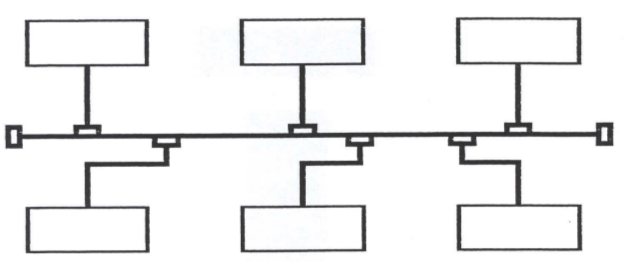
\includegraphics[width=2cm]{bus.png} &
    \includegraphics[width=2cm]{star.png} &
    \includegraphics[width=2cm]{circle.png} &
    \includegraphics[width=2cm]{tree.png} \\
    Full mesh & Bus & Star & Ring & Tree
\end{tabular}
    \caption{Different organisations.}
\end{figure}

\begin{itemize}
    \item \textbf{A full mesh}
    The most efficient, but needs $\frac{n \times (n-1)}{2}$ links, and every
    host has to manage $n-1$ interfaces which quickly becomes impossible.

    \item \textbf{Bus organisation}
    The danger is that if the bus' cable is ruptured, the network is divided
    which can be hard to maintain.

    \item \textbf{Star organisation}
    The node at the center of the star is vital for the network, but it permits
    centralisation of control in a single point. (\textit{It's an excellent
    control point and a good observation point.})

    It's a lot easier to maintain than a bus organisation.

    \item \textbf{Ring organisation}
    A link shuts down the entire network, which is why a dual-ring is often
    used.

    \item \textbf{Tree organisation}
    Allows for connecting a large amount of clients with very low cost.
\end{itemize}

\subsubsection{Sharing bandwidth}

Bandwidth sharing in networks is \textbf{max-min fair}. (Can't allocate more
bandwidth to a flow without reducing the bandwidth of another).

Multiple algorithms are explained in the Medium Access Control section,
\sectionref{medium_access_control}.

\subsubsection{Network congestion}

\textbf{Congestion} when $\sum \textnormal{demand} > \textnormal{capacity}$.

\paragraph{Congestion collapse}
Arrives when the network is slightly congested, and thus transmission is slowed
down. If a protocol such as \textbf{selective repeat} is used, the sender might
thing the packet has been loss and therefore send back a packet which only adds
onto the congestion.

To regulate congestion, one solution is to know the actual congestion so that
the hosts can adjust their accessible bandwidth to reduce congestion.

\subparagraph{$\to$} As long as the buffer isn't full, demand is less than
capacity and therefore the buffer just serves \textbf{to smooth} demands over
time, otherwise the demand is going to be higher than the available bandwidth,
which in turn leads to congestion.


\paragraph{Discard mechanism}
Packets can be discarded when the buffer is full, or rather when its size goes
up dramatically in order to prevent congestion. However, discarding a packet is
the last resort.

\begin{enumerate}
    \item \textbf{Discard the ingoing (tail drop)}: the most common one, but
    it tends to add on to the existing congestion and real-time applications
    suffer from this.
    \item \textbf{Discard the next outgoing (drop from front)}: smarter than
    it might seem since this packet has been there for a long time and surely
    the loss (due to congestion) has been detected beforehand.
    \item \textbf{Random early discard}: discards a random packet.
    (\textit{Allows for discarding packets from different flows proportional to
    their bandwidth.})
\end{enumerate}

\subparagraph{Remark:} Discarding a packet isn't the smartest solution since
it boils down to discarding a packet which has used up resources, when
resources are exactly what is missing in the first place.

\paragraph{Forward Explicit Congestion Notification}
For datagram networks, a bit is used to show whether the packet has passed
through a congested area, and if it has, the receiver sends a packet to inform
the sender of the degree of congestion (which is equal to
$\frac{n_{\textnormal{congested}}}{n_{\textnormal{total}}}$).

\paragraph{Backward Explicit Congestion Notification}
Identical technique for virtual networks, except for the fact that
acknowledgment is shown.

\paragraph{Control packet}
Allow the network node to send a \textbf{control packet} to the source to
indicate the current congestion level. Their usage is mainly restricted to
small networks because:
\begin{enumerate}
    \item In large networks this packet increases the network load when the
    network is congested.
    \item Network nodes are optimized for forwarding packets, not creating them.
\end{enumerate}

\paragraph{Scheduler mechanism}
Allows to attribute a FIFO queue for each flow and a round-robin chooses the
next packet.


\subsubsection{Distributing the load across the network}

\paragraph{Virtual network}
Here, when a host wants to send out information, they have to specify its
destination and sometimes the necessary bandwidth. They then get a response
telling them whether they can connect. This technique is named
\textbf{connection admission control}. (\textit{An example of usage is in
telephones.})

\paragraph{Datagram network}
The virtual network technique can't be used here because the host doesn't need
autorisation to send out packets. See \sectionref{congestion} for various
techniques for reacting to congestion.

\paragraph{Shared popular file}
\begin{itemize}
    \item \textbf{Save on multi server}: One server name known by the client
    and the client sends a \textsc{query} to know the address of the server.
    (\textit{Automatically, if there is different server the address can change
    for different people.})
    \item \textbf{Using a popular bittorent service}: Split the file into
    different blocks and the client needs all blocks to have the file. There is
    a \textbf{metadata} file that contains where each block can be downloaded.
    (\textit{Most deployments of bittorents allow the clients to participate
     in the distribution of the blocks.})
\end{itemize}

\subsubsection{Medium Access Control (MAC)}
\label{sec:medium_access_control}
The first of the 3 resources that need to be shared inside a network is the
link bandwidth (\textit{the 2 others are router processing time and router
buffers}).

\textbf{Collisions} happen when two hosts try to send a frame simultaneously.
They are the principal source of errors in Local Area Networks.

\paragraph{ }
There are 2 types of MAC:
\begin{itemize}
    \item \textbf{Deterministic} or pessimistic MACs: They ensure that there
    will be \emph{no} collision. They are more appropriate in networks where
    the load is constant (e.g. telephone, radio).
    \item \textbf{Stochastic} or optimistic MACS: They try to minimize the
    number of collisions. They are more appropriate in networks where the load
    has an on-off behaviour (e.g. internet).
\end{itemize}

\paragraph{\textbf{Deterministic MAC}}
The deterministic MACs are the following (the first three are \emph{static}
allocation methods).
\begin{itemize}
     \item[-] \textbf{Frequency Division Multiplexing}:
     In a wireless medium, we can give a different frequency for devices.
     \item[-] \textbf{Wavelength Division Multiplexing}:
     In an optical medium, we can give a different wavelength for devices.
     \item[-] \textbf{Time Division Multiplexing}:
     In any medium, we can just divide the time in separate slots and assign
     the slots to devices statically or dynamically.
     \item[-] \textbf{IEEE 802.4 (Token Bus Network)}:
     Transmit a token in a network with a bus topology. To transmit data, wait
     for the token and then transmit the data instead of the token. Once the
     data is transmitted, put the token back in the network.
     \item[-] \textbf{IEEE 802.5 (Token Ring Network)}:
     Same as 802.4 but with a ring topology.
     \item[-] \textbf{Deterministic Medium Acces Control (DMAC) }: Example
     with the Token Ring
     \begin{itemize}
          \item Nodes have two modes: listen mode where they forward the signal
          they receive, inserting a one bit delay and transmit mode where they
          have the token and they transmit data.
          \item There is a special node called \textbf{monitor} which ensures
          that the token always travels on the token ring (it inserts a token
          size delay).
          \item Nodes stop transmitting when they get their own bit. the
          beginning of the token is the beginning of the data frame so the node
          can know with a bit if it's a token or data.
          \item A station can't retain the token for more than Token Holding
          Time.
     \end{itemize}
\end{itemize}

\paragraph{\textbf{Stochastics MAC}}

\begin{itemize}
    \item[-] \textbf{[slotted] ALOHA}: First approach is ALOHA. When no ack is
    received, we wait a \textcolor{red}{random time} instead of a fixed time to
    \textbf{avoid synchronisation} with other hosts.

    A simple improvement is \textbf{slotted} ALOHA which divides the times into
    slots of the same size as the time required to transmit one frame.
    Transmisssions are only allowed to start at the beginning of a time slot.
    This avoids collision on part of a frame since that requires the frame to
    be completely retransmitted anyway.

\item[-] \textbf{[non-]persistent Carrier Sense Multiple Access (CSMA)}:
An improvement to ALOHA is \textbf{persistent} CSMA which senses the network
before sending a frame but does not wait a random time.

To avoid synchronisation with CSMA, \textbf{non-persistent} CSMA waits a random
time before sensing the network. If it is not free, it will wait a random time
before sensing it again.

\item[More] improvements can be made but depend on the technology.

\item[-] \textbf{CSMA/CD for IEEE 802.3 (Ethernet)}: On ethernet, a host is
able to detect a collision while it is listening.

If $\tau$ is the diameter of the network (the largest time between 2 hosts), we
know that if a frame of length $2\tau$ has a collision, the sending host
\textbf{will sense it} (as any other host by the way). We therefore enforce
$2\tau$ as the minimum frame size.

$\to$ Since Ethernet doesn't have many transmission errors, CSMA/CD does
\textbf{not use acknowledgment} to avoid the collisions they would cause. Also,
because the sender knows when there is a collision, it knows when a
transmission error occurs.

The time waited by the hosts when a collision is detected is random to avoid
synchronisation, is a multiple of $2\tau$ for the same reason as slotted ALOHA
and is selected in a range multiplied by 2 after each collision. This is called
a \emph{binary exponential back-off}.

\item[-] \textbf{CSMA/CA for IEEE 802.11 (WiFi)}

\begin{description}
    \item[\sifs{}]: This is required to \textbf{switch} between upload and
    download in a router.
    \item[\difs{}]: The channel must be idle \difs{} microseconds before a device
    can transmit \textbf{after the previous frame was received correctly}.
    \item[\eifs{}]: the time the device must sense the channel idle \textbf{after
    the previous frame was corrupted} before transmitting.
    \item \[\sifs{} < \difs{} < \eifs{}.\]
\end{description}

There is a \textbf{random} exponential \textit{backoff timer} in addition to
\difs{} or \eifs{} before sending a frame. (\textit{This timer is
frozen when the channel is busy!})

Another problem with wireless is the \textit{hidden station problem}, where you
don't receive the signal of another device (and therefore can't see when the
channel is busy).

To solve this, there are two control frames: \textsc{RTS} (ask for a delay
reservation) and \textsc{CTS} (to confirm reservation). (\textit{Small size to
minimize collisions.}) All hosts are informed of the reservation.

\begin{figure}[ht]
    \centering
    \includegraphics[width=6cm]{hiddenstation.png}
    \caption{Hidden station problem.}
\end{figure}

\end{itemize}

\subsubsection{Congestion control}
\label{sec:congestion}

To remove \strong{congestion collapse}, the hosts have to regulate their
transmission rate. (\emph{There are other mechanisms to regulate this such as
the one based around credits.})

\paragraph{Goals of congestion control} for a set of $i$ hosts:
\begin{itemize}
    \item Has to remove congestion, that is $\forall t \sum r_i(t) \leq R$.
    \item Efficiency, that is $\forall t \sum r_i(t) \approx R$.
    \item Fairness ($\to$ max-min fairnessis the ideal).
\end{itemize}

Such a mechanism can be implemented in the \textit{transport layer} or in the
the \textit{network layer}. (TCP/IP implements this in transport.)

\paragraph{Congestion control} is an algorithm that adjusts the rate of
congestion:
\begin{enumerate}
    \item \textbf{Multiplicative decreasing} if there is congestion:
    $\textnormal{rate} = \textnormal{rate} \cdot \beta, \quad \beta <1$.
    \item \textbf{Additive increasing} otherwise:  $\textnormal{rate} =
    \textnormal{rate} + \alpha, \quad \alpha>0$.
\end{enumerate}

\paragraph{Congestion control in window-based transport protocol}
Reducing the window size can reduce the congestion because a device cannot
send data faster than: \[\frac{\textnormal{Window}}{\textnormal{rtt}},
\textrm{ where window is current sending window}\]

\subparagraph{Limit window size}
\begin{itemize}
    \item[-] Review: \textit{swin} is the size of the sending window,
    \textit{rwin} is the size of the receiving window and now \textit{cwin} is
    the congestion window.
    \item[-] \textbf{Congestion window}: limits the sending window.
    \textit{swin} = $\min(swin,cwin)$
\end{itemize}

When starting, \textit{cwin} is set to one segment and it increases
(\textit{additive}) by one every RRT when there is no congestion, else it is
divided by two (\textit{multiplicative}).

\paragraph{Note: }
\begin{description}
    \item Congestion is detected when a packet is lost.
    \item Mild congestion: 3 duplicate acks ($\to$ Fast retransmit).
    \item Severe congestion: retransmission timer expires.
\end{description}

\subsection{The reference models}


\begin{table}[ht]
    \begin{tabular}{|c|c|c|c|}
        \hline
        Application & SDU     &                                        &  \\
        \hline
        Transport   & Segment & Connectionless unreliable              &
        connect to network  \\
                    &         & connection-oriented often reliable   & \\
        \hline
        Network     & Packet  & Unreliable                             &
        connect to network \\
        \hline
        Datalink    & Frame   & Reliable (if it uses ack and an error is
        detected) & directly connect to device \\
        \hline
        Physical    & Bit     & Unreliable                             &
        directly connect to device \\
        \hline
    \end{tabular}
    \caption{Reference models.}
\end{table}

\paragraph{TCP/IP reference model} The same but the physical layer and datalink
layer are combined into the link layer.

\paragraph{OSI Model} There is a session and a presentation layer before the
application layer. The session layer deals with the organisation and the
synchronization of the message/data exchanged with the presentation entity.
The presentation layer deals with representing the information.

\section{Protocols}

\subsection{Application layer}
An application uses connectionless or connection-oriented services and is
\textcolor{red}{identified} by a port number and a network address
(\textit{IPv4 or IPv6}). TCP is also called the byte-stream mode service and
UDP the datagram service.

\begin{description}
    \item IPv4: 32 bits wide.
    \item IPv6: 128 bits wide.
\end{description}

\subsection{DNS}

\begin{figure}[ht]
    \centering
    \includegraphics[width=10cm]{dnsheader.png}
    \caption{DNS header.}
\end{figure}
DNS usually runs above datagram service. The message is divided into five
parts. The first three are mandatory, the other two are optional. In the DNS
message header, there is an identifier to match requests to return inforrmation
on server authority (that is, who manages the server). A request is recursive
when the resolver recurses through the DNS hierarchy to retrieve its answer.
\paragraph{Resource Record}
\begin{itemize}
	\item[Time-to-Live] How long the client can keep the Resource Record inside its cache.
	\item[Type] Field in the record to specify either IPv4(A) or IPv6(AAAA).
\end{itemize}


DNS allows for obtaining the address which corresponds to a certain name, but
can also be reversed to obtain the name corresponding to a certain address.

\subsection{Electronic mail}

An \textbf{email system} is composed of:
\begin{itemize}
    \item A message format.
    \item Protocols: to exchange between host and server.
    \item Client software: to create/read mail.
    \item Software: to allow the server to efficiently exchange mail.
\end{itemize}

\begin{figure}[ht]
    \centering
    \includegraphics[width=10cm]{mail.png}
    \caption{Simplified mail architecture.}
\end{figure}

\subsubsection{Email messages}
Email messages are composed of two parts: a \textbf{header} (\textit{From*,
Date*, To*, Subject,  cc, bcc}) and a \textbf{body}. (* indicates mandatory
fields).

There is an empty line to separate header and body which contains only CR and
LF.

\subsubsection{Header field to support Multipurpose Internet Mail Extension
(MIME)}
New header lines support MIME\footnote{To add non-ASCII characters in mail
without breaking the email servers that were deployed at that time.}:
\begin{itemize}
    \item MIME-version: MIME version for encoding mail.
    \item Content-type: Datatype of the message:
        \begin{enumerate}
            \item multipart/mixed: the file contains independent parts (text,
            binary separated in the body by empty lines).
            \item multipart/alternative: same message but with different
            representations (e.g. text and HTML).
        \end{enumerate}
    \item Content-Transfer-Encoding: How the message is encoded and a second
    parameter explaining which string is used to delimit fields.
\end{itemize}
 A frequent encoding for email is \textbf{Base64} where sequences of bytes are
 encoded in groups of three bytes adb then each group is divided into six-bit
 fields that correspond to a character. (`=' is reserved for padding).

\subsubsection{The Simple Mail Transfer Protocol (SMTP)}

SMTP is a client/server protcolol and text-based protocol relies on the
connection-oriented service. (\textit{Server listens on port 25})
\paragraph{Note:} The DNS MX record of the DNS is used to find the destination
SMTP server.
Five agents are involved:
\begin{multicols}{2}
	\begin{itemize}
		\item Mail User Agent: email client.
		\item Mail Submission Agent: Process and forward.
		\item Mail Transmission Agent: Forward to other MTA or MDA.
		\item Mail Delivery Agent: Deliver to MUA destination.
	\end{itemize}
\end{multicols}
Each agent forwards to the next agent.
\paragraph{Working:}

\begin{tabular}{m{9cm}m{6cm}}
\begin{enumerate}
    \item The client opens transport connection with the server.
    \item Once connection is established, the client server exchanges
    \textit{greeting} messages (\textsc{EHLO}).
    \item After that, the email transfer phase can start: clients transfer one
    or more emails by indicating \textsc{MAIL FROM:} and \textsc{RCPT TO:}.
    \item At the end, the connection is closed (QUIT).
\end{enumerate}
&
\includegraphics[width=7cm]{stmp.png} \\
\multicolumn{2}{m{15cm}}{220: service ready, 221: connection close, 250:
action okay, 354: start mail, 3xx: need more information, 5xx: error.}
\end{tabular}

\subsubsection{The post office protocol (POP) }
POP runs above a connection-oriented service. (\textit{Server listens on port
110}), it allows a client to download all of his/her email from a server.

\paragraph{Working:}

\begin{tabular}{m{9cm}m{6cm}}
\begin{enumerate}
    \item Autorisation phase when the server verifies the client's credentials
    (\textit{username/password}).
    \item Transaction phase when the client downloads the message.
    \item Update phase that concludes the session.
\end{enumerate}
&
\includegraphics[width=7cm]{pop.png} \\
\multicolumn{2}{c}{+ok: accept, -ERR: error.}
\end{tabular}


\subsection{HTTP}
Uses hypertext links to link files together.

\paragraph{Three components of the \textbf{World Wide Web}}
\begin{enumerate}
    \item \textbf{Uniform Resource Identifiers}: A URI \strong{uniquely}
    identifies a resource on the World Wide Web.
    \item A standard document format: \textbf{HTML}, containing hypertext
    links.
    \item A standard protocol with efficient access to documents on the server:
    \textbf{HTTP} made of request(\textit{method, header, MIME document}) and
    responses(\textit{status line, header, MIME document}).
\end{enumerate}

\paragraph{\textbf{URI}} is divided up in three parts:
\begin{enumerate}
    \item A \textbf{protocol} for the application layer (\texttt{http://},
    \texttt{mailto:}, \texttt{ftp://}).
    \item \textbf{Authority} which is the IP address or DNS server where the
    file is located.
    \item A \textbf{path} to the file in UNIX format.
\end{enumerate}

\subparagraph{URI looks like this:}
\texttt{protocol://utilisateur@serveur:port/ressource}.

\paragraph{\textbf{HTML}}
Divided up in two parts: head and body.

\paragraph{\textbf{HTTP}}
Protocol is text-based and runs above a connection-oriented service. Contains:
\begin{enumerate}
    \item A \textbf{method} (\textit{GET, HEAD, POST}), a \textbf{URI} and a
    version of the HTTP.
    \item A \textbf{header} (specifies optional parameters).
    \item An optional MIME.
\end{enumerate}

\subparagraph{Persistent TCP connection}
An HTTP request has to be \strong{self-contained}. For this reason, HTTP1.0
would open a different connection for every HTTP request. HTTP1.1 introduced
\textbf{persistent TCP connections} via two new HTTP headers:

\begin{itemize}
    \item \textbf{Connection}: with \textit{Keep-alive or close} to specify
    what the client wants.
    \item \textbf{Keep-alive}: with the \textbf{maximum number} of requests
    that the server agrees to serve and the \textbf{timeout} after which the
    server will close an idle connection.
\end{itemize}

\paragraph{Preferences}
However, it is possible for servers to want to personalise responses according
to the client's preference. Three solutions come to mind:

\begin{enumerate}
    \item By forcing the client to authenticate themselves, (user/password is
    deprecated).
    \item By using HTTP headers such as \texttt{Accept-*}. In real use, this is
    however not used except for Accept-language by the browser.
    \item By using cookies in two headers: Cookie (\textit{request}) and
    Set-cookie (\textit{response}).
\end{enumerate}

\subsection{Remote procedure call}
Similar to calling a procedure inside code, except for the fact it happens on
the network.

\paragraph{Encoding data}
The first issue is encoding data. Two popular mechanisms exist: \textsc{xdr}
(\textit{more efficient}), \textsc{json} (\textit{more readable}),\ldots

\paragraph{Reaching the call}
The second issue is sending out data.

A simple mechanism is \textsc{json-rpc} which can be used both
connectionless or connection-oriented, containing:
\begin{itemize}
    \item a request: a \textbf{json-rpc} string indicating the version of the
    protocol, the name of a \textbf{method}, a structure containing the
    \textbf{params} and an \textbf{id}.
    \item a response: a \textbf{json-rpc} string indicating the version of the
    protocol, a \strong{result} or an error and an \textbf{id}.
\end{itemize}

\subsection{Internet transport protocols}
On the internet, the network layer provides an unreliable connectionless
service and an IP address to identify each host, with a maximum packet size
equal to $\SI{64}{\kilo\byte}$ of payload.

\subsection{The User Datagram Protocol (UDP)}
Unreliable connectionless transport service, runs on top of an unreliable
connectionless network service, which uses ports to allow communicating with
multiple applications and has the following characteristics:

\begin{itemize}
    \item SDUs have to be $< \SI{65467}{\byte}$.
    \item Does not guarantee the SDU is delivered.
    \item Can't deliver a corrupted SDU.
\end{itemize}

\paragraph{Header} = Source port (16), dest port (16), length (16) and checksum
(16)

\paragraph{Port:} 0--1023 (\textit{privileged}), 1024--49 151
(\textit{registered}), 49 152--65 535 (\textit{ephemeral})

\paragraph{Usage}
\textbf{UDP} is used when delay must be minimised or losses can be recovered by
the application itself. (\textit{Or real-time applications like interactive
videos.})

\subsection{The transmission control protocol (TCP)}
Bi-directional bytestream of a connection-oriented transport service, runs on
top of an unreliable connectionless network service.

(Window-based transport protocol using Go-Back-N).

\paragraph{Header:}
\begin{itemize}
    \item Source port (16), Destination port (16).
    \item Sequence number per byte (32), ack number (32), window size (16)
        \begin{itemize}
            \item[$\to$] TO make a reliable data transfer.
        \end{itemize}
    \item Flag: \textit{SYN, FIN, RST, ACK}.
    \item checksum (16).
    \item Length in world (4).
\end{itemize}

\subsubsection{TCP connection etablishment}
Three-way handshake using a sequence number, ack number and SYN/ACK/RST flag.

\begin{figure}[!ht]
  \centering
  \includegraphics[width=12cm]{tcpconnect.jpg}
  \caption{TCP connection.}
  \label{fig:tcpconnect}
\end{figure}

While connection is being established, the client/server negotiates different
options:
\begin{enumerate}
  \item The \textbf{MSS}, which is the size of the largest acceptable payload
  (\textit{at least 536}).
  \item Window size.
  \item Usage of SACK (Selective ACK) (information on out-of-sequence segments).
  \item A number of options where the client and the server both communicate
  what they want and support.
\end{enumerate}

\paragraph{Options encoding} is done with \textsc{TLV}, Type-Length-Value.

\paragraph{Robustness principle:} SYN can contain unknown options without
crashing, however, SYN+ACK can only contain (from these options) those options that we know and recognize (other options will be ignored).

\paragraph{Denial of service attacks}
A server maintains a TCB (transmission control block) which contains the state
of each connection's TCP entity. To avoid memory overflow, the TCB's size is
limited to 100.

\textbf{Denial of service attacks} try to render data on the network
unaccessible.

\textbf{SYN flood attack} merely has to flood the server with SYN to flood its
TCB, thus blocking everyone from establishing a connection with it.

\subparagraph{Solution:} Using client-side cookies to replace the server TCB.
However, this isn't entirely backward-compatible with the TCP option.

\subsubsection{TCP reliable data transfert}

For every TCP connection, a \textbf{TCB} (transmission control block) is
maintained with all necessary information to send and receive segments.

\paragraph{Segment transmission strategy}

Two radical solutions:
\begin{enumerate}
    \item Send when needed, but this could mean sending out a single byte of
    information, together with 20 header bytes, which is hardly ideal.
    \item Send whenever \textsc{mss} bytes of data have been filled.
\end{enumerate}

\subparagraph{Nagle's algorithm:} the packet is sent if it either fills up the
\textsc{mss}  or if an acknowledgment has just been received. (\textit{At least
every round trip time}).

\subsubsection{TCP window}

Negociating the window scaling factor ($0 \leq \textnormal{scaling}  \leq 14$)
is done at connection time, even if some implementations automatically adjust
its size.

\subsubsection{TCP retransmission}
\textbf{Go-Back-N} needs a good retransmission timer (\textsc{rtt} is a good
first guess even though it changes over time).
\begin{center}
\textsc{rtt} $\approx$ delay between the transmission of a segment and the
reception of an ack.
\end{center}

\paragraph{Measure RTT}
The issue is we don't know which segment the ack refers to (multiple identical
segments might have been sent).

To solve this, \textbf{timestamp options} are used:
\begin{itemize}
    \item \textbf{TS}: for example clock value.
    \item \textbf{TS} echo: last received \textsc{ts}.
\end{itemize}

Since there is no more ambiguity, the time value can be updated
($\textnormal{rtt} = \SI{3}{\second}$ at initialization).

\begin{align*}
\textnormal{srtt} \textrm{ (smoothed rtt mcomputed) } &=  (\alpha \times
\textnormal{srtt}) + (1-\alpha) \times \textnormal{rtt} \\
\textnormal{rto} \textrm{ (retransmission timedout) } &= \min(60, \max(1, \beta
\times \textnormal{srtt})).
\end{align*}

where rtt is the measured \texttt{RTT} and $60, 1$ are minimal/maximal bounds.

\subparagraph{Jacobson's algorithm:}
However, in a real world environment, this doesn't work too well. To solve this
problem, Jacobson proposed the following idea: rto is always initialised to
\SI{3}{\second}.
\begin{multicols}{2}
\begin{itemize}
    \item[-] For the first \texttt{RTT} value
        \begin{align*}
            \textnormal{srtt} &= \textnormal{rtt} \\
            \textnormal{rttvar} &= \frac{\textnormal{var}}{2} \\
            \textnormal{rto} &= \textnormal{srtt} + 4 \cdot \textnormal{rttvar}.
       \end{align*}

    \item[-] Otherwise
        \begin{align*}
        \textnormal{rto} &= \textnormal{srtt} + 4 \cdot \textnormal{rttvar} \\
        \textnormal{rttvar} &= (1-\beta) \times \textnormal{rttvar} + \beta
        \times \abs{\textnormal{srtt} - \textnormal{rtt}} \\
        \textnormal{srtt} &= (\alpha \times \textnormal{srtt}) + (1-\alpha)
        \times \textnormal{rtt}).
   \end{align*}
\end{itemize}
\end{multicols}

\paragraph{$\alpha, \beta$ value: }  $\beta = \frac{1}{4}, \alpha =
\frac{1}{8}$.

\subsubsection{Advanced retransmission strategy}

\paragraph{}
\textsc{tcp} uses \textbf{Go-Back-N} by default, and when the same timer has
expired, it is doubled (called \textit{exponential backoff}) until it reaches
\SI{60}{\second} after which it is declared unreachable.

\paragraph{Piggybacking} is used by \textsc{TCP} when there is a bidirectional
data transfer, which is rather rare.

\paragraph{Delayed acknowledgment strategy}
It is also possible to have performance issues when sending acks when they
serve no real purpose. Typically, a \textbf{delayed acknowledgment strategy}
can be implemented which makes sure an ack is sent every time a timer runs out
(\textit{a typical delay value is one second}) or when an out-of-sequence
segment is received because in that case the ack is of utmost importance.

\paragraph{Out-of-sequence}
It's really easy for the receiver to add a buffer to recover the
out-of-sequence segments without having to notify the sender.

\paragraph{Fast retransmit}
Currently, the timer has to end before a lost segment can be sent back. Another
method is to detect the error when three acks are received for the same
segment.

It does however require a \texttt{dubpacks} variable to be added to the
\textsc{tcb}.

\paragraph{Selective repeat}
One of the \textsc{tcp} options allows activating \textbf{SACKs} which allow us
to indicate which segments were received out-of-sequence. In this case, Fast
Retransmit is often used.

\subsubsection{TCP connection release}
Abrupt (\textsc{rst}) or gracefully (FIN, FIN+ACK).

\subsection{The stream control transmission protocol (SCTP)}
Alternative to \textsc{tcp} which offers the following characteristics:
\begin{enumerate}
    \item Efficiently supports \textbf{multihomed hosts}, that is multiple
    network interfaces. In \textsc{tcp}, there is a single IP address per
    interface, which means that if a user is connected via WiFi and the
    connection is dropped, mobile data can't recover instead.
    \item The possibility to send \textbf{messages} via bytestream.
    \item Partially-reliable, useful for timed delivery.
    \item A single real connnection with logical streams in order to avoid
    having to manage multiple connections.
\end{enumerate}

\subsubsection{Segment}
A segment is a header followed by a sequence of chunks.
\begin{figure}[ht]
    \centering
    \begin{tabular}{m{8cm}m{7cm}}
        \includegraphics[width=8cm]{sctpsegment.png} &
        \includegraphics[width=7cm]{sctpchunk.png}
    \end{tabular}
    \caption{SCTP segment/chunk format.}
\end{figure}

\paragraph{Header} = Source port number (16), dest port number (16),
verification tag (32) and checksum (32).

\paragraph{Chunk} = Type (8), flags (8), length (16) and value (32) to allow
for easy insertion of options. STCP, as opposed to \textsc{tcp}, is not limited
in its number of options. Its a good example of an easy to extend protocol.


\subsubsection{Connection etablishment}
Four-way handshake (to protect against ``Denial of service attacks'').

\begin{figure}[ht]
    \centering
    \includegraphics[width=6cm]{fourway.png}
    \caption{Four-way handshake.}
\end{figure}

\subsubsection{Reliable data transfer}

\begin{figure}[ht]
    \centering
    \begin{tabular}{m{8cm}m{8cm}}
    \includegraphics[width=8cm]{datachunk.png} &
    \includegraphics[width=8cm]{sackchunk.png}
\end{tabular}
    \caption{SCTP data/sack chunk format.}
\end{figure}

\paragraph{Data chunk}
Data is sent via \textbf{data chunks} which use a TNS as a sequence number
(increment by 1 for every data chunk). When a chunk is divided up into parts,
the \textsc{b} and \textsc{e} bits are used to specify the first and last chunk.

\paragraph{Sack chunk}
To guarantee arrival, a cumulative TNS ack is used (on chunck level and not
byte level). It also supplies information about the out-of-sequence chunks. Some
other differences include:
\begin{enumerate}
    \item Can supply information about the various ``holes'' in the reception
    buffer.
    \item Can give feedback about a duplicate chunk. (Points to a bad heuristic
    on the sender's behalf.)
\end{enumerate}

\subsubsection{Connection release}
Uses a three-way handshake to close the connection, or an \texttt{ABORT} chunk
to either refuse connection or close it immediately.

\subsection{UDP - TCP - SCTP}
\begin{table}[ht]
    \begin{tabular}{|c|c|c|c|c|c|}
    	   \hline
    	    Protocol& Reliablility&\# options&Mode&Establishment&Num seq\\
        \hline
        UDP & Unreliable   & x              & Stream-mode     &
        x                   & x \\
        \hline
        TCP & Reliable     & Option finie   & Stream-mode     & Three-way
        handshake & seq. = byte \\
            &              &                &  Single host
            &                     &  \\
        \hline
        SCTP & Reliable or & Option infinie & Message mode as & Four-way
        handshake & chunk \\
             & partially   & with chunk     & a stream mode
             &                    & \\
             &             &                & Multihomed host
             &                    & \\
        \hline
    \end{tabular}
    \caption{Differences between UDP, TCP and SCTP.}
\end{table}
\subsection{Congestion control}
The transport layer is where control happens.

TCP controls congestion by acting on the window size since a
connection can't send data faster than \[\frac{\textnormal{window}}{rtt}\quad
\textnormal{window} = \min(swin,rwin).\]

\paragraph{Congestion window}
\textbf{CWND} is stored in the \textsc{TCB} of every connection and the size of
the window is $\min(cwnd, rwin, swin)$.
\begin{itemize}
    \item[-] \textit{Additive increase}: every \textsc{rount trip time},
    \textsc{cwnd} is incremented by MSS bytes (Congestion Avoidance Phase).
    \item[-] \textit{Multiplicative decrease}: when congestion is detected,
    \textsc{cwnd} is decreased by a certain factor.
\end{itemize}

\paragraph{Initial value of cwnd:}
\textbf{MSS} bytes so as to not cause congestion of the network at its launch.
(This initial value has been rounded up to \SI{15}{\kilo\byte}.)


However, cwnd goes up slowly until it arrives to a value which uses the network
efficiently. To avoid this slow process, a \textbf{slow-start algorithm} is
used which doubles \textsc{cwnd} every RTT.

\paragraph{Detecting congestion} comes down to detecing packet loss.

\begin{itemize}
    \item \textit{mild congestion}: if fast retransmit is used (cwin divided
    by two).
    \item \textit{severe congestion}: when the transmission timer expires
    (ssthresh is divided by 2 and $\textnormal{cwin} = \textnormal{MSS}$).
\end{itemize}

\begin{figure}[ht]
    \centering
    \begin{tabular}{m{8cm}m{8cm}}
    \includegraphics[width=8cm]{severecongestion.png} &
    \includegraphics[width=8cm]{midlecongestion.png} \\
    \multicolumn{1}{c}{Severe congestion.} & \multicolumn{1}{c}{Middle
    congestion.}
\end{tabular}
    \caption{Congestion window when congestion is detected.}
\end{figure}

\subsubsection{Controlling congestion without losing data}
The main idea here is to detect congestion before actual packet loss by using an
\textbf{Explicit Congestion Notification}. (When a packet passes through a
congested router, the \textbf{CE} bit is set to 1 and when the receiver gets
this information they transmit it back to the sender in order for the latter to
adjust their rate.)

\begin{enumerate}
    \item In order to use this solution, \textbf{another bit} (ECT, ECN-capable
    transport) is needed to specify whether the packet uses \textbf{ECN} or
    not. If nothing is specified, and the router is congested, the ones that
    do not implement ECN are given priority.

        \begin{itemize}
            \item[$\to$] if the router is congested and the packet implements
            ECN, CE is set to 1, otherwise the packet is discarded.
        \end{itemize}
    \item If the protocol is reliable, the sender can be informed through an
    ack, either via a flag in the header or an option (TCP uses a flag, STCP
    uses an option).
        \begin{itemize}
            \item[$\to$] A variable keeps a value of 1 on the receiver end
            while received packets are marked as ``congested''.
        \end{itemize}
    \item Lastly, the sender and receiver know whether they are using a ECN via
    a TCP option during the connection three-way handshake.
\end{enumerate}

If the receiver detects congestion, the next sent packets will have this
information (to avoid it being lost if the ack gets lost).

\paragraph{Router algorithm}
Two types of routers, either with a single FIFO or multiple FIFOs and a round
robin scheduler.

Instead of measuring the buffer's fullness at a given moment in time, an
average is taken. On top of that, every packet has a certain probability of
being marked ``congested'', and the higher the average fullness is, the higher
this probability becomes (Random Early Detection).

\paragraph{}
When multiple queues are present this probability is computed independently to
guarantee its correctness.

\subsubsection{Modeling TCP congestion control}
To show the factors that affect the performance of TCP, if $p$ is the segment
loss ratio then $\frac{1}{p}$ is the number of successfully transferred
segments.

\begin{figure}[ht]
    \centering
    \includegraphics[width=9cm]{modelingtcp.png}
    \caption{Evolution of the congestion window with regular losses.}
\end{figure}

\begin{description}
    \item The number of segments that are sent during a cycle is in yellow:
    $A = \frac{3 \times W^2}{8}$.
    \item But by definition, $A = \frac{1}{p}$ so: $W = \frac{k}{\sqrt{p}}$
    \item The throughput (\textit{bytes/sec}) is the number of segments
    transmitted divided by the duration of the cycle:
    \[\textnormal{Throughput} = \frac{A \times
    \textnormal{MSS}}{\textnormal{time}} \quad \approx \frac{k \times
    MSS}{\textnormal{rtt} \times \sqrt{p}}.\]
\end{description}

This is an important result which shows that:
\begin{itemize}
    \item TCP connections with \textbf{smaller rtt} have higher throughput than
    ones with higher rtt when losses occur (\textit{unfair}).
    \item TCP connections that use a \textbf{large MSS} can achieve a higher
    throughput than ones with shorter MSS (\textit{unfair}). Most hosts use the
    same $\textnormal{MSS} = \SI{1460}{\byte}$.
\end{itemize}

\paragraph{Conclusion:} $\textnormal{Throughput} <
\min(\frac{\textnormal{window}}{\textnormal{rtt}}, \frac{k \times
\textnormal{MSS}}{\textnormal{rtt} \times \sqrt{p}})$
Maximum throughput depends on the maximum window size and rtt if there are no
losses, otherwise it depends on the MSS, rtt and loss ratio.

\subsection{Network layer}
Three types of datalink layers:
\begin{enumerate}
    \item Directly a physical link from the physical layer.
    \item Local Area Network.
    \item Non-Broadcast Multi-Access (used to emulate a LAN with only unicast).
\end{enumerate}

\paragraph{LAN}
In a LAN, every host is identified by a datalink layer address (\textbf{MAC
address}).

A LAN supports broadcast and multicast datalink layer addresses. A frame sent
to the \textbf{multicast} address of the LAN is sent to all the participants in
the group. The \textbf{broadcast} address is used to send out messages to
everyone.

\subsubsection{IP version 6}
Soon, IPv4 won't be able to accommodate for all addresses anymore, which is why
another solution is needed.

\begin{tabular}{m{2.5cm}m{10cm}}
    Assumptions: &
    \begin{itemize}
        \item[-] Adress encoded on 128 bits.
        \item[-] IPv6 format header can easily be parsed by hardware device.
        \item[-] Able to configure IPv6 address automatically.
        \item[-] Security.
    \end{itemize}
\end{tabular}

\paragraph{IPv6 addressing architecture}
Scalability of a network layer protocol depends on its addressing architecture.

IPv6 supports \textbf{unicast, multicast and anycast}.

\paragraph{\textbf{Unicast}}:

\begin{tabular}{m{8cm}m{7cm}}
    \begin{itemize}
        \item Global routing prefix that is assigned to the \textbf{Internet
        Service Provider}.
        \item Subnet id identifies a customer of the ISP.
        \item Interface id.
    \end{itemize}
    &
    \includegraphics[width=8cm]{unicast.png}
\end{tabular}

\paragraph{ }
\textbf{Hierarchical} address allocation allows for minimising the amount of
routes known to the router. It therefore only knows the route for certain
address blocks (\textit{$2^{128}$ grouped in $2^{64}$ subnets!}).

Two types of address allocation:
\begin{itemize}
    \item \textit{provider independent} (PI): For companies connected to at
    least two ISPs. Address blocks are given out independently of the ISP.
    \item \textit{provider aggregatable} (PA): Depends on the ISP.
\end{itemize}

The drawback with \textbf{PA} addresses is that when your provider changes, all
the addresses you use in a PA address block also change.

\paragraph{Size IPv6 address}
\texttt{/32} = Internet Service Provider, \texttt{/48} = single company,
\texttt{/56} = small user site, \texttt{/64} = single user, \texttt{/128} =
rare. (No more than one host attached to a prefix.)

\paragraph{Usage of the IPv6 prefix}
\textbf{Longest prefix match} assures the route that has the best match with
the address is the one that is used.

Note:\texttt{::/0} matches with all and is therefore the \textit{default
route}.

\paragraph{\textbf{Unique Local Unicast}}
The ULA address is an \texttt{fc00::/7} and is similar to an IPv4 address. The
address isn't necessarily unique and a router doesn't forward a ULA.

As opposed to local unicast links, it doesn't necessarily need to have the same
link.

\paragraph{\textbf{Link Local Unicast}}
The address starts with \texttt{fe80::/64}, followed by 64 interface bits. Used
when two hosts on the same link (or LAN) want to exchange a packet. The router
can't forward a packet with a local unicast link. (\textit{Used when regular
IPv6 isn't an option, that is, an isolated LAN.})

\paragraph{\textbf{Multicast}}
Allows for sending a packet to all people in a same LAN group.

\begin{figure}[ht]
    \centering
    \includegraphics[width=8cm]{multicast.png}
    \caption{Multicast address.}
\end{figure}


\paragraph{\textbf{IPv6 packet format}}

\begin{figure}[ht]
    \centering
    \includegraphics[width=12cm]{ipv6format.png}
    \caption{IPv6 packet format.}
\end{figure}

\subparagraph{Header}(\SI{40}{\byte}) = Payload length (16 bits), Hop limit:
\textit{limit of the router that can forward the packet} (8 bits) and Next
header (8bits) + Version (4bits) + SRC (128b) + DST (128b) + Traffic (8bits
ECE/ECT).

\subparagraph{No checksum}
There is no checksum in the IPv6 packet header since there is already a
checksum on the \textbf{frames} at the datalink layer level.
Adding an (expansive) checksum will detect memory corruption errors inside the router,
which hardly happen.

\subparagraph{Next header}
Indicates the next header, such as a transport layer header (\textit{UDP=17,
TCP=6, SCTP=132}) or an IPv6 option since the packets can have multiple
headers. An option also has the \textit{next header} field.

\subparagraph{Options}
Contain a next header, a length and an \textbf{opt field} which indicates what
the receiver should do in case of an unknown option:
\begin{itemize}
    \item[-] 00: continues without worrying about the option.
    \item[-] 01: discards the packet.
    \item[-] 10: returns a control packet.
\end{itemize}

\subparagraph{Fragment option}
In IPv6, fragmentation is done by the sender and not by the router. The router
discards the packet and send an error message to the sender if the packet is
too big.

A fragmented packet contains:
\begin{itemize}
    \item[-] the offset (13) of the fragmentation;
    \item[-] next header (8) (\textit{because it's an option});
    \item[-] a flag: 0 = last fragment;
    \item[-] a field to identify the \emph{original} packet. It must make sure
    not to use the same one for MSL seconds.
\end{itemize}

\subparagraph{Note:}
Packets can be sent from first to last or in reverse order. The second solution
allows for the receiver to know the size of the packet (and thus the necessary
buffer). When a fragment is received, a timer is started and if all fragments
haven't arrived by the end of this timer, the packet is considered lost.

\paragraph{Loose source} IPv6 option to determine which route to take (router
addresses are specified). Isn't used because of security concerns.

\subsubsection{ICMP version 6}
\textit{Internet Control Message Protocol} version 6 is used in IPv6 packets.
(next header = 58) to transmit messages to the sender. There are two types of
messages:

\begin{itemize}
    \item Error messages:
        \begin{enumerate}
            \item Destination unreachable (0: no route, 1: firewall refuse, 2:
            sender used link-local address to reach global unicast address, 3:
            address unreachable, 4: port unreachable);
            \item Packet too big;
            \item Time exceeded;
            \item Parameter problem.
        \end{enumerate}
    \item Information messages: when a host receives an \textit{Echo request},
        it has to respond with an \textit{Echo reply}.
\end{itemize}

\paragraph{PathMTUDiscovery}
Use of ICMP segment to discover the MTU of the path. Then adjust MSS to avoid
fragmentation.

\subsection{The IPv6 subnet}
Every interface on a device is identified by a unique MAC address\footnote{MAC
address blocks are allocated to manufacturers.}.

Thanks to this uniqueness, two hosts connected on a LAN have a unique address.

\paragraph{Broadcast:} the packet is delivered to all devices attacked to the
datalink network.

\paragraph{Multicast:} just like a broadcast, except the interface knows
whether a packet is destined to it or not (\textit{based on a logical address}).

Potentially, all IPv6 nodes are capable of capturing frames destined to
different multicast addresses.

\subsubsection{Interactions between IPv6 and datalink layer}

\paragraph{In an internetless LAN,} hosts take on an IP address thanks to
\textbf{link-local addresses}: with MAC addresses, \texttt{fe80::/64} is chosen.

\paragraph{If the LAN is connected to the internet,} the \textbf{Neighbor
Discovery Protocol} (part of ICMPv6) is used to determine the others' addresses.

\paragraph{Neighbor Discovery Protocol (NDP)}
Care must be taken since IPv6 addresses have been configured \textbf{manually}.

\begin{enumerate}
    \item Sends out a \textbf{ICMPv6 Neighbor Solicitation} (NS) with the IPv6
    address in question.
    \item The receiver responds with a \textbf{ICMPv6 Neighbor Advertisement}
    with its IPv6 and MAC addresses.
    \item As it is receiving the ICMPv6 NA, it stores the IPv6-MAC link in its
    \textbf{NDP table} (mapping between IP address and MAC).
\end{enumerate}

\subparagraph{Note:} ICMPv6 NS can also be used in unicast to know whether a
host is reachable. On top of that, the ICMPv6 NA is stored temporarily in the
cache and when it expires, the address has to be revalidated.

\paragraph{Duplicate Address Detection algorithm} makes it possible to not have
two identical IPv6 addresses. In order to do this, it sends an \textbf{ICMPv6
NS} in unicast to its address, and if it doesn't receive a response, it is
unique.

\paragraph{\textbf{Automatically configure IPv6 addresses}}
There are two protocols: SLAAC and DHCPv6.

\subparagraph{Stateless Address Auto-Configuration (SLAAC) }
\begin{enumerate}
    \item A device creates its \textbf{link-local address} with
    \texttt{fe80::/64} and \SI{64}{\bit}, part of which comes from the MAC.
    \item It verifies its uniqueness by sending out an \textbf{ICMPv6 NS} with
    its link-local in multicast.
    \item To know the \textit{prefix IPv6 subnet}, the router regularly sends
    ICMPv6 \textbf{Router Advertisements}, multicast on \textbf{ff02::1}
    \footnote{Corresponds to all reachable hosts.} containing:
        \begin{itemize}
            \item[-] \textit{Cur hop limit}: maximum number of intermediate routers (usually 64).
            \item[-] \textit{Router lifetime}: estimated time where the router
            is the default router.
            \item[-] \textit{Reachable time and Retrans timer}: used to
            configure the NDP protocol usage for the subnet hosts.
        \end{itemize}

        A lot of \textbf{options} can be added to Router Advertisement messages:
        \begin{itemize}
            \item \textbf{MTU} option: indicates the maximum size of what can
            be transmitted \textbf{without} fragmentation on the subnet.
            \item \textbf{Prefix} option: gives the prefix size and its length,
            and the estimated lifetime of the prefix.
        \end{itemize}
    \item IPv6 address = Prefix + 64 identification bits.
    \item Sends an \textbf{ICMPv6 NS} to its IPv6 to assure uniqueness.
\end{enumerate}

\subparagraph{Notes:} A device can send an ICMPv6 Router Solicitation to the
router via \textbf{ff01::2}\footnote{Corresponds to all reachable routers.} to
ask for an ICMPv6 RA if it considers the delay to be too long.

\subparagraph{Dynamic Host Configuration Protocol (DHCP)}
Uses a DHCP server. This server has a set of addresses and listens on port 67.
\begin{itemize}
	\item When a host connects, they sends a \textbf{DHCP request} in UDP to
     all other DHCP servers.
	\item The server captures the request, and sends a \textbf{DHCP reply}
     with a non-assigned IP address. This reply also contains the lifetime of
     the address to force address renewal. Addresses can be reused.
\end{itemize}

\paragraph{Multi router on subnet}
Thanks to \textbf{ICMPv6 Redirect Messages}, it's possible for hosts to
automatically learn new routes:

\begin{itemize}
    \item[-] When a router has to forward back a packet, it has to send an
    ICMPv6 RM which indicates the packet has to be sent by another router.

    \item[-] Updates its forwarding table (\textit{a timer is often associated
    to this new router to discard the router after a certain period of time}).
\end{itemize}


\subsection{Routing in IP networks}
Two classes of protocols between different domains to efficiently exchange
information.

A big difference between \textbf{intra} and \textbf{inter} domain are the
\textit{routing policies} used by each domain.

In a domain, all routers are equal and the best router is chosen based on
several criteria: time, number of intermediaries and bandwidth size.

\subsection{Intradomain routing}
Exchanges information about the reachable destinations \textbf{in} the domain.
\textit{RIP} is a \textbf{distance vector} protocol and \textit{OSPF}
uses \textbf{link-state routing}.

\subsubsection{RIP}
Routers periodically exchange RIP messages (inside \textbf{UDP} segments).

To accelerate the process when a router boots, it can send a \textbf{RIP
request} by multicast to \texttt{ff02::9} (\textit{to query the routing
tables}).

All those who receive such a request respond by sending out their routing table
and a sequence of \textbf{RIP responses}.

\paragraph{Note:}
Routers periodically (\SI{30}{\second}) send one or more RIP responses
with the distances vectors summarising the routing table. However, this caused
the router to synchronise and sometimes flooded it. Nowadays, a random wait
time between 15 and 30 is added.

\subsubsection{OSPF}
With link-state routing, it's very costly for big networks to store all of the
network in memory.

\begin{tabular}{m{10cm}m{5cm}}
    \begin{itemize}
        \item \textbf{Border router}: Router attached tp multiple areas.
        \item \textbf{Internal router}.
        \item \textbf{Area}: Routers know the topology of their area and how to
        reach the backbone area.
        \item \textbf{Backbone area}: area that groups the \textbf{border
        routers} and those that aren't in an area.
    \end{itemize}
    &
    \includegraphics[width=5cm]{area.png}
\end{tabular}

It's worth noting border routers need manual configuration.

\paragraph{Area}
Routers exchange link-state packets with everyone in the area.

\paragraph{Inter-area}
Inter-area routing is done by switching distance vector protocols to prevent
routers from having additional costs to reach routers from a different domain.

\paragraph{LAN}
When routers boot in a LAN, they elect a (\textbf{Designated Router}) so as to
not have to exchange HELLO packets between all routers. The routers can only
exchange HELLOs with the DR; it represents the LAN. (\textit{The LAN topology
looks like a full mesh of point-to-point links connected to the DR router.})

\subsubsection{Shortest path}
Intradomain protocols choose the shortest path. It is possible for two paths to
have the same cost. In that case, two possibilities arise:
\begin{itemize}
    \item always use the same (\textit{and only put this one in the forwarding
    table});
	\item use the different paths:
	\begin{itemize}
		\item via a round robin, but this means using different paths for
          packets from a same flow (TCP connection) and thus potentially
          increasing the out-of-sequence arrivals;
        \begin{center}
            (\textit{out-of-sequence $\to$ duplicate ack $\to$ fast retransmit
            $\to$ congestion.})
        \end{center}

		\item use a round robin for every flow, via a hash value of the
          packet tuple. The same interface (path) will be used for packets from
          the same flow.
          \[hash(NextHeader, IP_{src}, IP_{dst}, Port_{src}, Port_{dst} ) \mod
          N.\]
          $N$ is the number of outgoing interfaces on the equal cost paths.
	\end{itemize}
\end{itemize}

\subsection{Interdomain routing}
Exchanges information between domains. This information is an aggregation of
the routers' information and domains are thus considered as black boxes.

A \textit{content-rich} subdomain is a domain that contains hosts that
mainly receive packets. (Google,\ldots)

\subsubsection{Connected link}
\begin{itemize}
    \item \textbf{Private peering link} allows to link two domains. For
    performance reasons, multiple physical links are established between
    domains.
    \item \textbf{Internet eXchange Point} A less costly solution is to connect
    them via an IXP. The IXP contains a LAN where all routers are connected.
\end{itemize}

\begin{figure}[ht]
    \centering
    \includegraphics[width=8cm]{exchange.png}
    \caption{Internet eXchange Point.}
\end{figure}

\subsubsection{Connection cost}
The \textbf{cost} of a route is very important in interdomain routing whereas
in intradomain routing, performance is more important.

\begin{figure}[ht]
    \centering
    \includegraphics[width=5cm]{peering.png}
    \caption{Peering relationships.}
\end{figure}

There are two types of relations between domains.
\begin{itemize}
    \item \textbf{customer $\to$ provider}: the customer pays for his domain to
    be distributed on the Internet. (\textit{The reciprocal of this is the
    provider sharing all routes it knows.})
    \item \textbf{Shared cost}: this happens when domains have similar sizes.
    \textit{We don't want a packet passng through a shared cost to not be
    destined to the domains after this link.}

        $\to$ Via a shared cost, a domain only announces its internal routes
        and the links with its clients.
    \item \textbf{Sibling}: they exchange routes in both directions (often
    routers from the same company).
\end{itemize}

\subsubsection{Interdomain routing policy}
\begin{itemize}
    \item \textbf{Import filter}: specifies the neighbour's acceptable routes
    for every link. (\textit{The non-acceptable ones are ignored and never used
    for forwarding packets.})
    \item \textbf{Export filter}: specifies for every link the routes that can
    be announced to the neighbour.
    \item \textbf{Ranking algorithm}: chooses the best route towards the prefix
    destination amongst the ones the domain received.
\end{itemize}

\begin{figure}[ht]
    \centering
    \includegraphics[width=11cm]{policies.png}
    \caption{Import export policies example.}
\end{figure}

\subsubsection{The Border Gateway Protocol (BGP)}

In the BGP every domain is identified by a unique \textit{Autonomous System}
number (AS).

BGP doesn't send its full routing table but does it incrementally, that is, by
sending out the ones that changed.

On top of that, BGP uses TCP to guarantee the correct delivery of BGP messages.

\paragraph{BGP session}

\paragraph{Etablishment} has to be done manually for security reasons.

\paragraph{Messages}

\begin{enumerate}
    \item \textit{OPEN}: when connection is established, the session is
    initialised and the options are negotiated.
    \item \textit{NOTIFICATION}: to close the session.
    \item \textit{UPDATE}: notifes of a route changement. It's the most
    important message and in order for the protocol to be efficient, the
    message should minimise the number of bits sent.
    \item \textit{KEEP ALIVE}: notifes nothing has changed (to make sure the
    router is still alive).
\end{enumerate}

\paragraph{BGP update} = \{IP prefix removed\}, \{IP prefix added\},
\{AS-Path\}.

\subparagraph{ } A route which is sent first has to pass through the
\textit{export filter}, and a received route has to pass through the
\textit{import filter}. A BGP router is composed of 4 datastructures:

\begin{itemize}
	\item Adj-RIB-In: the routes the router now knows but hasn't filtered yet.
	\item Local-Routing-Information Base: routes learned after import filter.
	\item Fowarding Information Base: mapping between destination and better
     route.
	\item Adj-RIB-Out: route the router teaches to the neighbour after the
     export filter.
\end{itemize}

\paragraph{The BGP decision process}
On top of the import/export filters, there is an algorithm that decides the
best route. This choice is made based off of the BGP attributes attached to
each route.

\paragraph{Local-pref}
The first attribute of this algorithm is the local-preference, which is
attributed according to the import filter (highest value is preferred).

\subparagraph{Cheap link}
It's possible to implement the preference of a cheap link rather than another via
the local-pref by defining the values in the import filter.

\paragraph{Local-pref with customer $\to $provider and shared cost}
\begin{enumerate}
    \item High local-pref for the routes learned by the customer
    (\textit{provider $\to$ customer}).
    \item Medium local-pref for shared-cause.
    \item Low local-pref for the routes learned by the provider.
    (\textit{customer $\to$ provider}).
\end{enumerate}

\paragraph{BGP convergence}
Certain routing policies can interfere with each other and theoretically lead
to infinite ``ping-pong''.

\paragraph{ }
BGP convergence isn't always guaranteed and verifying global convergence is
NP-complete. % is it P though ;-)

\paragraph{Guideline to guarantee BGP convergence}
\begin{enumerate}
    \item The \textit{customer $\to$ provider} graph is acyclic.
    \item AS prefers a route received from a customer rather than a shared-cost.
\end{enumerate}

\subsubsection{Global structure of the Internet}
Domains can be divided up into 4 categories w.r.t. their roles and positions in
the AS topology:
\begin{itemize}
	\item Tier-1: the kernel of the Internet, the domains without a provider.
	\item Tier-2: customer of Tier-1, they're the smaller customers and share
     costs with other T2.
	\item Tier-3: customer of Tier-1 and Tier-2 (stub domains or small ISPs).
	\item Large content providers: Large datacenter, they produce large parts
     of the exchanged data over the Internet. Customers of T1 or T2 but are
     usually in shared-cost with T1 or T2 via IXP.
\end{itemize}

\subsection{Datalink layer technology}

\subsubsection{The point to point protocol}
We limit ourselves to the study of protocols which are often used for
\textbf{transport of IP packets} between hosts and routers connected by
point-to-point links.

\paragraph{\textbf{Serial Line IP} (SLIP):}
It's a technique used for character stuffing applied to IP packets using two
special characters:
\begin{itemize}
    \item \textsc{END}: at the beginning and end of a packet.
    \item \textsc{ESC}: in front of an END if it is part of the information
    to be transmitted.
\end{itemize}

\begin{tabular}{cm{11cm}}
    \underline{Limitations} of SLIP:
    &
    \begin{itemize}
     \item Only supports IP packet transmission.
     \item Manual configuration of addresses between host and router.
    \end{itemize}
\end{tabular}

\subparagraph{Note:} SLIP was mainly used for links $\leq \SI{20}{Kps}$ on
which \textbf{TCP/IP header compression} techniques were essential.
(\textit{Headers already took a lot of time.})

    $\implies$ Consecutive segment redundancy is exploited to compress.

\paragraph{\textbf{Point-to-Point protocol} (PPP):}
Supports IP and other protocols of the network layer for different transmission
lines. It uses bit stuffing or character stuffing according to the environment
where the protocol is used.

PPP is a family of 3 protocols that are used simultaneously:
\begin{enumerate}
    \item the \textit{Point-to-Point Protocol}: framing technique for
    transporting packets in the network layer;
    \item the \textit{Link Control Protocol}: used to negotiate options and to
    authenticate the session (\textit{username/password, \ldots});
    \item the \textit{Network Control Protocol}: different for every protocol
    of the network layer, it allows negotiating the protocol-specific options
    (\textit{IPv4's NCP negotiates the IPv4 address}).
\end{enumerate}

\subparagraph{Frame:}
The Address (8) and Control (8) fields are present for compatibility reasons.
The Protocol (16 bits) field contains the ID of the type of protocol used for
the PPP frame transport. PPP supports packets of variable size but LCP can
negotiate a maximum packet size.

\begin{figure}[!ht]
    \centering
    \includegraphics[width=10cm]{ppp_frame_format.png}
    \caption{Format of a PPP frame.}
\end{figure}

\begin{center}
\textit{PPP supplies an access dial-up (commuted line) to the ISPs. This access
to the Internet is done via the Extensible Authentication Protocol (EAP)
using a password. With the arrival of the Asymmetric Digital Subscriber Lines
(ADSL) and wanting to reuse their authentication/facturation system, IETF has
developped specifications for PPP frame transport on other networks than
point-to-point.}
\end{center}

\subsubsection{Ethernet}

\paragraph{Ethernet standard 1980:}
\begin{itemize}
    \item \textbf{Speed}: \SI{10}{\mega\bit\per\second}
    (\textit{\SI{3}{\mega\bit\per\second} in 1970}).
    \item \textbf{Slot time}: \SI{51.2}{\milli\second} (\textit{minimum frame
    size $= \SI{64}{\byte}$}).
        \begin{itemize}
            \item[$\to$] Equal to twice the time needed for an electronic
            impulse to travel the maximum distance between two nodes. Waiting
            for this slot time allows for collision detection in CSMA/CD.
        \end{itemize}
    \item \textbf{Frame format}:
        \begin{itemize}
            \item \textbf{Dest address} (48 bits): multicast, broadcast and
            unicast. Is placed at the beginning of the frame so that the
            receiver can easily find out whether it's destined to them.
            \item \textbf{Source address} (48 bits): only unicast.
            \item \textbf{Type} (16): type of the packet transported on the network layer, \textbf{CRC} (32).
            \item $\SI{46}{\byte} < \textnormal{\textbf{Payload}} <
            \SI{1500}{\byte}$.
        \end{itemize}

        An Ethernet frame begins with a preamble used by the
        physical layer to synchronize clocks.
    \item \textbf{Adresses}:
        \begin{itemize}
            \item \textbf{unique} global address (MAC address) on \SI{48}{\bit}
            (\textit{makes allocating big blocks of addresses possible for the
            manufacturer});
            \item definition of broadcast and multicast addresses.
        \end{itemize}
\end{itemize}

\begin{figure}[!ht]
  \centering
  \includegraphics[width=9cm]{ethernet_address_format.png}
  \caption{MAC address format.}
\end{figure}

\paragraph{ }
An Ethernet network supplies \textbf{unreliable connectionless service}
(\textit{with unicast, multicast et broadcast}) such that:
\begin{itemize}
    \item very high probability of successful delivery ($\to$ use of CSMA/CD);
    \item frame transmission in order ($\to$ Ethernet network topology = shared
    bus).
\end{itemize}

\begin{figure}[!ht]
    \centering
    \includegraphics[width=6cm]{impact_of_frame_length_in_ethernet.png}
    \caption{Usage percentage as a function of frame size.}
\end{figure}

\begin{table}[ht]
    \centering
  \begin{tabular}{c|c|c|c|c|c}
  Name & Speed & Cable length & Cable type & Repeaters & Network topology \\
  \hline
  10Base5 & \SI{10}{Mbps} & \SI{500}{\metre} & Coaxial cable & Yes & Shared
  bus\\
  10Base2 & & \SI{185}{\metre} & Coaxial cable && Shared bus\\
  10BaseF & & & Optical link && \\
  10BaseT & & & Twisted cable && Star\\
  \end{tabular}
  \caption{Different physical layers defined for Ethernet.}
\end{table}


\paragraph{The introduction of twisted cables} lead to two major changes for
Ethernet:
\begin{itemize}
    \item The physical topology of the network (star-shaped).
    \item The necessity of inserting hubs to create this topology.
\end{itemize}

\paragraph{Hub:}

\begin{tabular}{m{10cm}m{5cm}}
     A hub is a relay on the physical network layer that
    \begin{itemize}
        \item receives an electrical signal on an interface;
        \item transmits on all other interfaces;
        \item is capable of converting electrical signals from two separate
        physical network layers (10BaseT$\to$10Base2).
    \end{itemize}
    &
	\includegraphics[width=5cm]{ethernet_hub.png}
\end{tabular}

To create a complex network with hubs, care has to be taken in different points:
\begin{enumerate}
    \item the network topology has to be a tree;
    \item collisions can happen $\to$ CSMA/CD;
    \item the extent of networks is limited by the slot time.
\end{enumerate}

\begin{figure}[!ht]
    \begin{center}
    \includegraphics[scale=0.3]{hierarchical_ethernet_network.png}
    \caption{A hierarchical Ethernet network made of hubs.}
    \end{center}
\end{figure}

\paragraph{Fast Ethernet}
is a LAN technology that makes it possible to reach up to \SI{100}{Mbps} by
using optical fiber. Two constraints:
\begin{itemize}
    \item has to support twisted cables (\textit{in the physical layer, coaxial
    cables would have been preferred but are harder to maintain});
    \item has to use the same frame format as with \SI{10}{Mbps} (because
    originally, this \SI{100}{Mbps} link was used as a link between two
    \SI{10}{Mbps} links).

        $\implies$ to preserve CSMA/CD: slot time = \SI{5.12}{\micro\second}.
\end{itemize}

\paragraph{\textbf{Ethernet switches}}
Another solution to get better performance in Ethernet LANs is by making hubs
intelligent.

\paragraph{Switch:}
\textit{intelligent hubs} capable of acting on the datalink
layer, analysing the destination address of every frame and forwarding in the
destined direction.
In this document, the words ``switch'' and ``bridge'' are used interchangeably,
although the latter term is more general.

\begin{figure}[!ht]
    \centering
    \begin{tabular}{cc}
        \includegraphics[width=6cm]{ethernet_switches.png} &
        \includegraphics[width=6cm]{switch_mac_address_table.png}
    \end{tabular}
    \caption{Ethernet switches and MAC address table.}
\end{figure}

\subparagraph{Switch forwarding table}
\begin{itemize}
    \item The forwarding table links the MAC address and the port to be
    forwarded to.

    \item MAC address (48 bits) usage, an Ethernet LAN is \textit{plug and
    play}. (\textit{As soon as you're connected you can start exchanging
    information.})

        \begin{itemize}
            \item[$\to$] Needs automatic switch table configuration.
        \end{itemize}

    \item With switches, the host only receives frames that are destined to
    them (\textit{unicast, multicast and broadcast}) as well as frames the
    switch doesn't know the destination of.

    \item[$\color{red}\bullet$] \textcolor{red}{Denial of service attack} The
    size of MAC tables is limited, a host can send a lot of frames with random
    sources and thus flood the switch.
        \begin{itemize}
            \item [$\to$] the switch has to broadcast every received frame, and
            thus the attacker gets all the frames.
        \end{itemize}
\end{itemize}

By combining \textbf{MAC  address  learning} and the forwarding algorithm, tree
networks without loops can be generated (no TTL, nor HopLimit).

(\textit{However, a tree is dangerous: in case of an issue with a link, the
network is divided up into two parts.})


\paragraph{Spanning Tree Protocol}
Allows for reducing the network to a \textbf{Spanning Tree}.
\begin{itemize}
    \item Bridges exchange BPDUs to create the spanning tree. The BPDUs are
    sent with multicast destination \textsc{ALL\_BRIDGES}.
    \item The smallest \SI{64}{\bit} identifier (lower 48 bits for the MAC
    address, higher 16 to allow the admin to influence the network) is chosen
    as the \textbf{root}, and the branches are composed of the shortest paths
    allowing every bridge in the network to be reached.
\end{itemize}

\subparagraph{BPU} ($\coloneqq \langle \textnormal{R, c, T, P} \rangle$)
contains:

\begin{itemize}
    \item the identifier of the root bridge (R);
    \item the cost of the shortest path between the bridge sending the BPDU and
    the root (c);
    \item the id of the bridge sending the BPDU (T);
    \item the port number of the bridge that sent the BPDU (p).
\end{itemize}

\subparagraph{Priority vector} $V[q] = \langle \textnormal{T, c} +
\textnormal{cost(q), T, p, q} \rangle$.

\subparagraph{Port}
Every port of the bridge is either a \textbf{root, designated} or
\textbf{blocked} port. A \textbf{root port} is the one closest to the root
bridge.

\begin{table}[ht]
    \begin{center}
    \begin{tabular}{|c|c|c|c|}
        \hline
        State of the port & BPDU reception & BPDU sending & Dataframe managing
        \\
        \hline
        Blocked & YES & NO & NO \\
        Root & YES & NO & YES \\
        Designated & YES & YES & YES \\
        \hline
    \end{tabular}
    \end{center}
    \caption{BPDU transmission in function of port state.}
\end{table}

\subparagraph{Function}

\begin{itemize}
    \item Every bridge listens to the BPDUs on its ports.
    \item For received BPDUs, the \textbf{priority vector} associated to the
    port where the BPDU is coming from is computed and the \textbf{best for
    each port} is stored.
    \item The root bridge is found by looking at the smallest identifier in the
    priority vector table:
        \begin{enumerate}
            \item the root bridge at $\langle \textnormal{R,O,R,p} \rangle$;
            \item the other bridges at $\langle \textnormal{R, c, S, p}
            \rangle$ know their root port (the one with the best priority
            vector).
        \end{enumerate}
    \item A port is designated if the bridge BPDU is better than the port's
    priority vector, otherwise it is blocked.
    \item[$\to$] R: root bridge, S: bridge ID, c: cost of the best priority
    vector, p: number of the port the BPDU originates from.
\end{itemize}

\subparagraph{When the version is stable,} the root bridge regularly sends out
its own BPDU which is received on the root port of the bridges that are
directly connected to the root.

\begin{itemize}
    \item Bridges listen on the blocked port, but if the network topology is
    stable, no BPDUs should arrive there.
    \item When computing the Spanning Tree, \textbf{no data} is transmitted
    over the network.

    After the spanning tree, the MAC learning algorithm starts.
\end{itemize}


\subparagraph{Failure recovery}
Bridges, ports and links can fail in an Ethernet network with bridges: when it
happens, the Spanning Tree has to be recomputed. In order to detect these
failures, BPDUs are regularly sent (BPDUs have two fields: age and maximum age).
\begin{itemize}
    \item $\textnormal{Age}=0$ for the root bridge and goes up one for every
    bridge it passes through.
    \item Switches store the age and increment it by one every second. If the
    maximum age is reached, a failure has occurred and the STP has to be
    recomputed.
\end{itemize}

\paragraph{Virtual LANs} are a set of ports and one or more bridges. A bridge
can manage multiple LANs separately and uses the MAC learning algorithm on
every VLAN without sharing their respective information.

\begin{figure}[ht]
    \begin{center}
      \includegraphics[width=9cm]{virtual_local_area_networks.png}
      \caption{Three Virtual Area Networks connected by bridges.}
    \end{center}
\end{figure}

To allow bridges to distinguish between VLANs, every VLAN gets an ID in every
exchanged frame header. This header is inserted directly after the MAC
address in the Ethernet frame (before EtherType).
\begin{figure}[!ht]
    \begin{center}
    \includegraphics[width=14cm]{header_vlan.png}
    \caption{VLAN header (802.1q).}
    \end{center}
\end{figure}

\begin{itemize}
    \item The Protocol tag is set to \texttt{0x8100}, which allows the receiver
    to detect the header's presence.
    \item The Priority Code Point (PCP) allows frame priorities to be defined.
    \item The C field allows compatibility between Ethernet and Token Ring
    networks.
    \item The last field is the VLAN identifier. (0 = not a VLAN; 4095 is
    reserved.)
\end{itemize}

\subsubsection{802.11 Wireless networks}
The radio spectrum is a limited resource shared by all. It's regulated by
international institutions and governments to avoid interference. The only
non-reglementary exception are ISM waves (Industrial, Scientific and Medical).
The \num{2400}-\SI{2500}{\giga\hertz} band is used for WiFi as well as
microwaves, bluetooth,\dots{} (thus interference is possible).

\paragraph{Standard 802.11}
IEEE created this standard for wireless networks (WiFi):
\begin{center}
\begin{tabular}{|c|c|c|c|c|}
\hline
Standard & Frequence & Typical bit rate & Maximum bandwidth & Reach
(\si{\meter})
inside/outside \\
\hline
802.11 & \SI{2.4}{\giga\hertz} & \SI{0.9}{Mbps} & \SI{2}{Mbps} & 20/100 \\
802.11a & \SI{5}{\giga\hertz} & \SI{23}{Mbps} &\SI{54}{Mbps} & 35/120 \\
802.11b & \SI{2.4}{\giga\hertz} & \SI{4.3}{Mbps} & \SI{11}{Mbps} & 38/140 \\
802.11g & \SI{2.4}{\giga\hertz} & \SI{19}{Mbps} & \SI{54}{Mbps} & 38/140 \\
802.11n & 2.4-\SI{5}{\giga\hertz} & \SI{74}{Mbps} & \SI{150}{Mbps} & 70/250 \\
\hline
\end{tabular}
\end{center}

WiFi uses CSMA/CA and the same architecture/frames as Ethernet.

The architecture of WiFi networks is different than the one for LANs. There are
two types of WiFi networks:
\begin{itemize}
    \item independent/adhoc: when it isn't connected to the Internet (WiFi
    printers,\dots);
    \item infrastructure: contain one or more access points attached to a LAN
    (often Ethernet) which is connected to the Internet.
\end{itemize}

The maximum theoretical payload in 802.11 is 2324 bytes but the standard is
limited to 1500.

\begin{figure}[!ht]
    \centering
    \begin{tabular}{cc}
        \includegraphics[width =6cm]{wifi_infrastructure.png} &
         \includegraphics[width=6cm]{wifi_access_point.png}\\
         802.11 network infrastructure. & WiFi access point.
     \end{tabular}
\end{figure}

\begin{figure}[!ht]
    \centering
    \includegraphics[width=12cm]{wifi_data_frame_format.png}
    \caption{802.11 dataframe format.}
\end{figure}

802.11 dataframe format:
\begin{itemize}
    \item Frame Control: indicates the frame type (data, RTS/CTS/ ack,
    management frames,\dots), whether the frame is sent from a LAN,\dots
    \item Duration: allows reserving transmission time (ack transmission time +
    \sifs{} for data; 0 for multi/broadcast).
    \item Sequence Control: has a sequence number incremented for every
    dataframe.
    \end{itemize}

There are three address fields:
\begin{enumerate}
    \item the MAC address of the access point;
    \item the MAC address of the WiFi source;
    \item the LAN final destination address.
\end{enumerate}

\paragraph{Unreliable connectionless service}
Despite the use of acknowledgments, the 802.11 layer only supplies unreliable
connectionless services like Ethernet. The acknowledgments are used to minimize
the probability of frame duplication, but don't guarantee data delivery (high
probability but no guarantee).

\paragraph{Encapsulation}
IP encapsulation on 802.11 adds 6 bytes to the 802.11 header, 4 bytes for
LLC/SNAP and 2 bytes of Ethernet Type (IP or ARP).

\begin{figure}[!ht]
\begin{center}
  \includegraphics[width=12cm]{ip_over_wifi.png}
  \caption{IP packet encapsulated in an 802.11 WiFi frame.}
\end{center}
\end{figure}

\section{Algorithms}
\lstset{keepspaces=true, morekeywords={isin, each},
keywordstyle=\color{red!70}, commentstyle=\color{blue!60},
breaklines=true}
   \subsection{MAC Address Learning by bridges}
	  \begin{center}
	  \framebox{\begin{minipage}{0.9\linewidth}
	     \lstinputlisting[language=Python]{mac_address_learning.py}
	  \end{minipage}}
	  \end{center}

    \subsection{Distance vector reception}
	  \begin{center}
	  \framebox{\begin{minipage}{0.9\linewidth}
	     \lstinputlisting[language=Python]{reception_of_distance_vector.py}
	  \end{minipage}}
	  \end{center}

    \subsection{Aloha}
	  \begin{center}
	  \framebox{\begin{minipage}{0.9\linewidth}
	     \lstinputlisting[language=Python]{aloha.py}
	  \end{minipage}}
	  \end{center}

    \subsection{Basic CSMA}
	  \begin{center}
	  \framebox{\begin{minipage}{0.9\linewidth}
	     \lstinputlisting[language=Python]{basic_CSMA.py}
	  \end{minipage}}
	  \end{center}

    \subsection{CSMA/CD final solution}
	  \begin{center}
	  \framebox{\begin{minipage}{0.9\linewidth}
	     \lstinputlisting[language=Python]{csma_cd_final_solution.py}
	  \end{minipage}}
	  \end{center}

    \subsection{Sender side CSMA/CA}
	  \begin{center}
	  \framebox{\begin{minipage}{0.9\linewidth}
	     \lstinputlisting[language=Python]{csma_ca_sender.py}
	  \end{minipage}}
	  \end{center}

    \subsection{Window-based congestion control}
	  \begin{center}
	  \framebox{\begin{minipage}{0.9\linewidth}
	     \lstinputlisting[language=Python]{window_based_congestion_control.py}
	  \end{minipage}}
	  \end{center}
	  \begin{center}
	  \framebox{\begin{minipage}{0.9\linewidth}
	     \lstinputlisting[language=Python]{AIMD_in_tcp.py}
	  \end{minipage}}
	  \end{center}

\subsection{TCP connection and deconnection}

\begin{figure}[!ht]
    \centering
    \includegraphics[width=10cm]{cofsm.png}
    \caption{TCP connection finite state machine.}
\end{figure}
\begin{figure}[!ht]
    \centering
    \includegraphics[width=10cm]{decofsm.png}
    \caption{TCP deconnection finite state machine. Timeout is 2*MSL.}
\end{figure}

\biblio


\end{document}
